\documentclass[master]{project_report}
\usepackage{url}
\usepackage{enumitem}
\usepackage{array}
\usepackage{placeins}
\usepackage{booktabs}
\usepackage{tabularx}
\usepackage{amsmath}
\usepackage{longtable}
\usepackage{pdfpages}

\title{
    Recreation and Wellness Intranet \\
    Manage Your Health Inc.
}

\author{
    Karan Goel - 7836685 \\
    Banin Sensha Shrestha - 8447196 \\ 
    Kushal Rimal - 8735876 \\ 
    Dipesh Baral - 8712785 \\ 
    Affan Mehmood - 8228851 
}


\submissionDate{}{}{2024}
\degree{System Analysis and Project Management} 

\begin{document}


\frontmatter

\makeatletter
\renewcommand{\@chapapp}{Part}
\makeatother

\mainmatter
%% Your chapters start here
\fancyhead[RO]{\textit{Part1}}
\chapter{Project Integration Management}

Our first step in ensuring the successful delivery of this project to MYH is to gain a comprehensive understanding of their primary goals and objectives. This part provides an overview of the main objectives, initial proposals, and business case studies that have been developed in consultation with the MYH.

\section{Case Study}

Manage Your Health, Inc. (MYH) is a global healthcare provider ranked among the Fortune 500. With over 25,000 employees worldwide, including 20,000 full-time and 5,000 part-time workers, MYH is committed to cutting internal costs, enhancing cross-selling of products, and leveraging new web technologies to foster collaboration among employees, customers, and suppliers, thereby enhancing the delivery of healthcare products and services.

MYH has identified three potential projects in line with their strategic objectives:

\begin{enumerate}[label=\textbf{\arabic*.}]
    \item \textbf{Health Coverage Costs Business Model:} This project involves developing a secure application to model and analyze healthcare expenses. It requires an initial investment of \$100,000 and is projected to save \$20 annually for each full-time employee.
    
    \item \textbf{Web-Enhanced Communications System:} The goal of this project is to implement a web-based system that streamlines the development and delivery of products. With a development cost of \$3 million, the system is expected to save \$2 million annually, notwithstanding ongoing maintenance costs.
    
    \item \textbf{Recreation and Wellness Intranet Project:} This initiative aims to launch an intranet application to enhance employee health and wellness, potentially reducing healthcare premiums and saving \$30 per employee each year through better health outcomes.
\end{enumerate}

MYH requests a preliminary analysis to determine which project best meets their strategic goals and asks for a detailed business plan for the chosen proposal.

\section{Project Analysis}

In response to the request from MYH, we initiated a preliminary analysis of the proposed projects. 

\subsection{Objectives Analysis}

The analysis began with an understanding of the strategic goals of MYH. These objectives were elucidated through comprehensive discussions with MYH's visionary leaders. The key strategic goals derived from these discussions are summarized in Table \ref{tab:myh_goals}.

\begin{table}[h]
    \centering
    \begin{tabular}{|c|p{10cm}|}
    \hline
    \textbf{Goal} & \textbf{Description} \\
    \hline
    Reduce-Cost & Aim to decrease internal costs to enhance efficiency and boost profitability. \\
    \hline
    Business-Growth & Increase market penetration and revenue through enhanced cross-selling opportunities. \\
    \hline
    Develop & Improve collaboration among employees, customers, and suppliers with new web-based technologies, thereby optimizing the development and delivery of healthcare products and services. \\
    \hline
    \end{tabular}
    \caption{Strategic Goals of Manage Your Health, Inc.}
    \label{tab:myh_goals}
\end{table}

\FloatBarrier

This structured approach allows us to align each project proposal with MYH's strategic objectives, facilitating an informed decision-making process for developing the subsequent business plan.

\subsection{Proposal Analysis}

Once the objectives were established, our team conducted a comprehensive analysis of each proposal to ensure they aligned with MYH's goals. We focused on several key metrics, assigning different weights to each criterion based on its importance:

\begin{itemize}
    \item Tie to business strategy - 10\%
    \item Upfront cost - 25\%
    \item Potential net savings - 25\%
    \item Realistic technology - 15\%
    \item In-house expertise - 10\%
    \item Potential resistance - 15\%
\end{itemize}

The findings of our analysis are summarized in Table \ref{tab:project_com}, providing a clear comparison of how each proposal measures up against the set criteria.

\begin{table}[h]
    \centering
    \caption{Comparison of Project Criteria and Their Impact}
    \label{tab:project_com}
    \begin{tabularx}{\textwidth}{>{\hsize=0.7\hsize}X>{\hsize=0.5\hsize}X>{\hsize=1.2\hsize}X>{\hsize=1.3\hsize}X>{\hsize=1.3\hsize}X}
    \toprule
    \textbf{Criteria} & \textbf{Weight} & \textbf{Health Coverage Costs Business Model} & \textbf{Web-Enhanced Communications System} & \textbf{Recreation and Wellness Intranet Project} \\
    \midrule
    Tie-to business strategy & 10\% & Reduce-Cost (1/3) & Business-Growth, Develop (2/3) & Reduce-Cost (1/3) \\
    Upfront cost & 25\% & \$100,000 & \$3,000,000 & \$200,000 \\
    Potential net savings & 25\% & \$1,600,000 & \$6,000,000 & \$2,400,000 \\
    Realistic technology & 15\% & Data Analysts needed to analyze the premiums of current and past employees linked to 10 different insurance companies. & The project is highly achievable with modern technology, as we all have experience with similar systems. & The project is highly achievable with modern technology, as we all have experience with similar systems. \\
    In-house expertise & 10\% & Organization might need to hire more experienced Data Analysts, even though we have expert developers to implement the application to analyze the data. & New components to be implemented and new services to be provided, such as delivery services, customer support, and suppliers management, necessitate hiring quite a few staff. & Project is easy to implement with proper guidance from a Team Lead. \\
    Potential resistance & 15\% & Project might not face much resistance since the application is relatively easy to build. & Project might not face much resistance since the application is relatively easy to build. & Senior employees might resist involvement in recreational programs due to greater responsibilities like family care. Other employees might also show disinterest. \\
    \bottomrule
    \end{tabularx}
\end{table}

\FloatBarrier

\subsection{Weighted Model} \label{sec:wm}

To further analyze our findings, we quantified the results from Table \ref{tab:project_com} to create a weighted model, as shown in Table \ref{tab:project_com_2}.

\begin{table}[h]
    \centering
    \begin{tabularx}{\textwidth}{>{\hsize=0.7\hsize}X>{\hsize=0.5\hsize}X>{\hsize=1.2\hsize}X>{\hsize=1.3\hsize}X>{\hsize=1.3\hsize}X}
    \toprule
    \textbf{Criteria} & \textbf{Weight} & \textbf{Health Coverage Costs Business Model} & \textbf{Web-Enhanced Communications System} & \textbf{Recreation and Wellness Intranet Project} \\
    \midrule
    Tie to business strategy & 10\% & 50 & 70 & 60 \\
    Upfront cost & 25\% & 70 & 35 & 85 \\
    Potential net savings & 25\% & 70 & 30 & 90 \\
    Realistic technology & 15\% & 60 & 85 & 75 \\
    In-house expertise & 10\% & 55 & 40 & 80 \\
    Potential resistance & 15\% & 80 & 85 & 60 \\
    \midrule
    \textbf{Total} & 100\% & 66.5 & 52.75 & 78 \\
    \bottomrule
    \end{tabularx}
    \caption{Comparison of Project Criteria and Their Impact (Weighted Model)}
    \label{tab:project_com_2}
\end{table}

\begin{figure}[ht]
    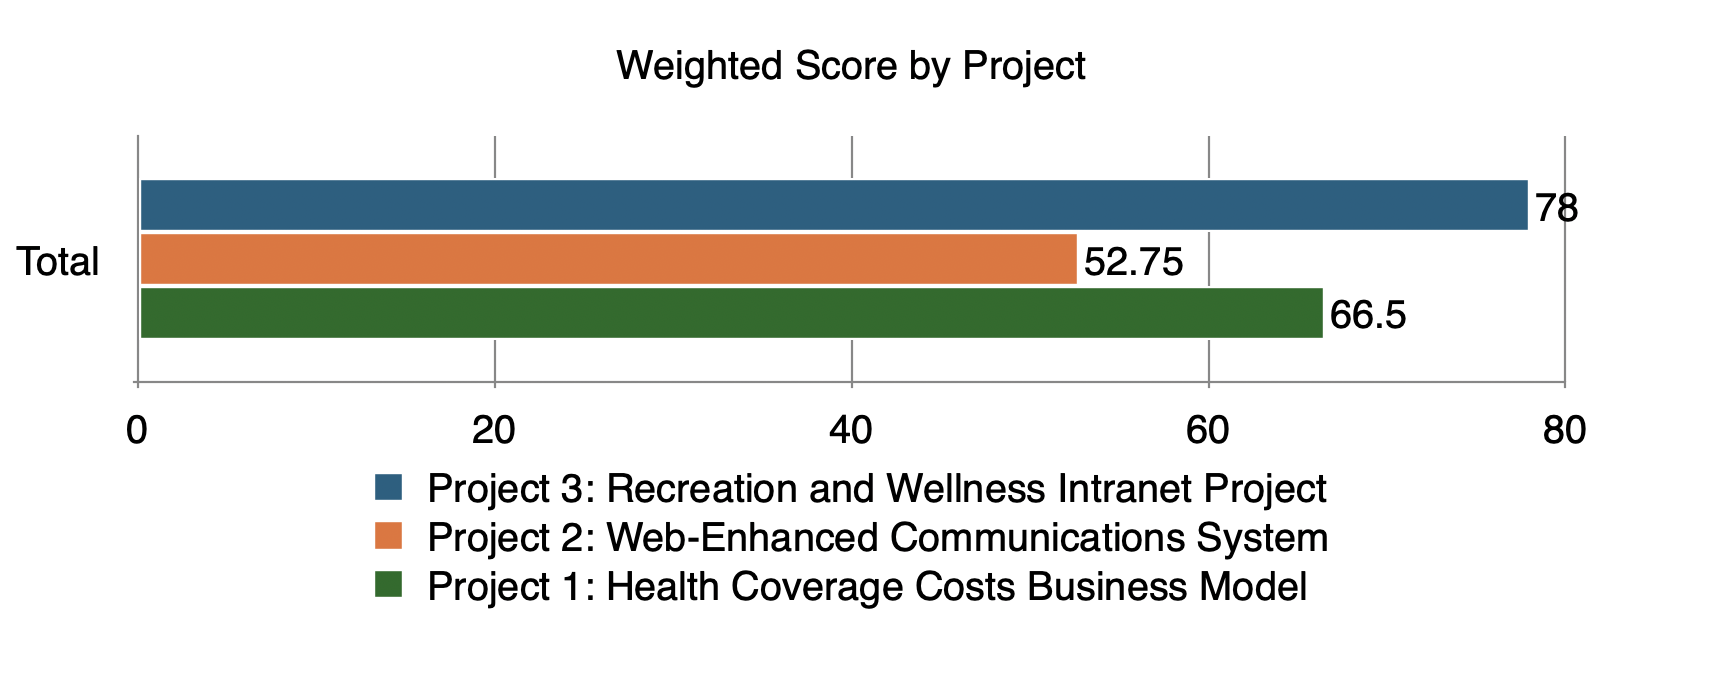
\includegraphics[width=\textwidth]{images/wsm.png}
    \caption{Weighted Score Model}
    \label{fig:wsm}
\end{figure}

The chart depicted in Figure \ref{fig:wsm} provides a visual representation of the evaluation model. From this chart, we can see that \textbf{Project 3: Recreation and Wellness Intranet Project} is the most preferred, followed by \textbf{Project 1: Health Coverage Costs Business Model}. This visual aids in understanding the relative preferences based on the weighted scoring of each project.

\subsection{Financial Analysis} \label{sec:fa}

To enhance our project selection process, we conducted a financial analysis to ensure that the chosen projects provide maximum benefit to MYH. Our team evaluated the Net Present Value (NPV) and Return on Investment (ROI) for each project to verify alignment with financial objectives and to ensure optimal returns. The detailed metrics and results of this analysis are summarized in the subsequent sections, providing a clear basis for our project recommendations.

\subsubsection*{Net Present Value (NPV)}
Net Present Value (NPV) is a financial metric used to evaluate the profitability of an investment or project. It represents the difference between the present value of cash inflows and the present value of cash outflows over the investment's lifetime. NPV is calculated using the formula:

\[
\text{NPV} = \sum_{t=0}^{n} \frac{C_t}{(1 + r)^t}
\]

where:
\begin{itemize}
    \item \( C_t \) represents the cash flow at time \( t \),
    \item \( r \) is the discount rate,
    \item \( t \) is the time period (usually in years),
    \item \( n \) is the total number of periods.
\end{itemize}

This formula discounts each of the cash flows back to their present value and then sums them up. A positive NPV indicates that the projected earnings exceed the anticipated costs, thus making it a potentially profitable investment.

\subsubsection*{Return on Investment (ROI)}
Return on Investment (ROI) is a financial metric used to measure the efficiency of an investment or to compare the efficiencies of several different investments. ROI measures the amount of return on an investment relative to the investment's cost, calculated as:

\[
\text{ROI} = \left(\frac{\text{Total Benefits} - \text{Total Costs}}{\text{Total Costs}}\right) \times 100\%
\]

where:
\begin{itemize}
    \item \(\text{Total Benefits}\) represents the total cash inflows from the investment,
    \item \(\text{Total Costs}\) represents the total cash outflows for the investment.
\end{itemize}

ROI is expressed as a percentage; a higher ROI means the investment gains compare favorably to its cost. It is used to evaluate the efficiency of an investment or compare the efficiencies of several different investments.

\subsubsection*{Financial Analysis of Projects}
The NPV and ROI calculations for the projects are detailed and summarized in Table \ref{tab:financial_analysis}. This table provides insights into the financial viability and potential profitability of each project, aiding in the decision-making process.

\begin{table}[ht]
    \centering
    \caption{Financial Analysis for Three Projects}
    \label{tab:financial_analysis}
    \begin{tabular}{lcccccc}
    \toprule
    \textbf{Item} & \textbf{Year 0} & \textbf{Year 1} & \textbf{Year 2} & \textbf{Year 3} & \textbf{Year 4} & \textbf{Total} \\
    \midrule
    \multicolumn{7}{c}{\textbf{Project 1: Health Coverage Costs Business Model}} \\
    \midrule
    Benefits & \$0 & \$400,000 & \$400,000 & \$400,000 & \$400,000 & \$1,600,000 \\
    Cost & \$100,000 & \$0 & \$0 & \$0 & \$0 & \$100,000 \\
    Cashflow & -\$100,000 & \$400,000 & \$400,000 & \$400,000 & \$400,000 & \$1,500,000 \\
    \textbf{NPV(D=8\%)} & \multicolumn{5}{c}{\textbf{\$1,134,121.05}} \\
    \textbf{ROI} & \multicolumn{5}{c}{\textbf{1500\%}} \\
    \midrule
    \multicolumn{7}{c}{\textbf{Project 2: Web-Enhanced Communications System}} \\
    \midrule
    Benefits & \$0 & \$2,000,000 & \$2,000,000 & \$2,000,000 & \$0 & \$6,000,000 \\
    Cost & \$3,000,000 & \$600,000 & \$600,000 & \$600,000 & \$600,000 & \$5,400,000 \\
    Cashflow & -\$3,000,000 & \$1,400,000 & \$1,400,000 & \$1,400,000 & -\$600,000 & \$600,000 \\
    \textbf{NPV(D=8\%)} & \multicolumn{5}{c}{\textbf{\$154,553.58}} \\
    \textbf{ROI} & \multicolumn{5}{c}{\textbf{11\%}} \\
    \midrule
    \multicolumn{7}{c}{\textbf{Project 3: Recreation and Wellness Intranet Project}} \\
    \midrule
    Benefits & \$0 & \$600,000 & \$600,000 & \$600,000 & \$600,000 & \$2,400,000 \\
    Cost & \$200,000  & \$0 & \$0 & \$0 & \$0 & \$200,000  \\
    Cashflow & -\$200,000  & \$600,000 & \$600,000 & \$600,000 & \$600,000 & \$2,200,000 \\
    \textbf{NPV(D=8\%)} & \multicolumn{5}{c}{\textbf{\$1,654,885.28}} \\
    \textbf{ROI} & \multicolumn{5}{c}{\textbf{1100\%}} \\
    \bottomrule
    \end{tabular}
\end{table}


\subsection{Project Selection}

After a thorough analysis of each project, considering both financial metrics (Section \ref{sec:fa}) and qualitative criteria (Section \ref{sec:wm}) we made a final decision on project selection for MYH.

\begin{itemize}
    \item \textbf{Project 1: Health Coverage Costs Business Model}
    \begin{itemize}
        \item \textbf{NPV}: \$1,134,121.05
        \item \textbf{ROI}: 1500\%
        \item \textbf{Decision}: Project 1 is appealing for selection due to its high ROI and substantial positive NPV, indicating significant profitability and efficient capital utilization but requires careful consideration of the additional staffing needs and its modest strategic tie.
    \end{itemize}

    \item \textbf{Project 2: Web-Enhanced Communications System}
    \begin{itemize}
        \item \textbf{NPV}: \$154,553.58
        \item \textbf{ROI}: 11\%
        \item \textbf{Decision}: Not recommended for immediate selection due to its lower ROI and marginal NPV, suggesting limited profitability and efficiency.
    \end{itemize}

    \item \textbf{Project 3: Recreation and Wellness Intranet Project}
    \begin{itemize}
        \item \textbf{NPV}: \$1,654,885.28
        \item \textbf{ROI}: 1100\%
        \item \textbf{Decision}: Project 3 offers a very high ROI and the highest NPV among the evaluated projects, ensuring excellent profitability and effective capital use. It presents a balanced option with moderate costs, significant expertise availability, and high feasibility with current technology, though it might face resistance impacting its implementation.
    \end{itemize}
\end{itemize}

Based on the comprehensive analysis of financial metrics along with the qualitative assessments, \textbf{Project 3: Recreation and Wellness Intranet Project} stands out as the optimal choice. This project not only demonstrates substantial financial returns but also aligns with technological feasibility and existing in-house expertise. Although there may be some resistance from senior employees, its moderate initial investment and significant long-term benefits warrant its selection. The project's strategic alignment with enhancing employee engagement and wellness further supports its potential for positive organizational impact.


\section{Business Case}
This section presents the business case for \textbf{Project 3: Recreation and Wellness Intranet Project}, proposed by Manage Your Health Inc. (MYH). 

The business case was developed based on the objectives, mission statement, goals, project phases, and financial and market analyses of the project. The results are summarized in Table \ref{tab:project_summary}. The detailed business case prepared by the project manager is presented below.


\begin{longtable}{|p{0.25\textwidth}|p{0.7\textwidth}|}
    \caption{Business case for Recreation and Wellness Intranet Project} \label{tab:project_summary} \\
    \hline
    \textbf{Section} & \textbf{Details} \\
    \hline
    \endfirsthead
    
    \multicolumn{2}{c}%
    {\tablename\ \thetable\ -- \textit{Continued from previous page}} \\
    \hline
    \textbf{Section} & \textbf{Details} \\
    \hline
    \endhead
    
    \hline
    \endfoot
    
    \hline
    \endlastfoot
    
    \textbf{Project Overview} & 
        \begin{itemize}
            \item \textbf{Project Manager:} Tony Prince
            \item \textbf{Client:} Manage Your Health Inc.
            \item \textbf{Duration:} 6 months
            \item \textbf{Budget:} \$200,000
        \end{itemize} \\
    \hline
    \textbf{Executive Summary} & 
        Aims to improve employee health and reduce healthcare costs by engaging employees in wellness and recreational programs, targeting savings of at least \$30 per employee per year. \\
    \hline
    \textbf{Mission Statement} & 
        To empower and engage employees in enhancing their health and well-being through accessible digital wellness solutions. \\
    \hline
    \textbf{Objectives} & 
        \begin{enumerate}
            \item Reduce healthcare costs by improving employee health.
            \item Enhance employee productivity and morale through structured wellness programs.
            \item Offer a tailored intranet solution to promote health management.
        \end{enumerate} \\
    \hline
    \textbf{Project Phases} & 
        Initiation, Planning, Execution, Monitoring and Control, Closure, and Post-Project Evaluation. Each phase includes specific tasks and resource allocations. \\
    \hline
    \textbf{Financial Appraisal} & 
        Project targets net savings of \$30 per employee per year, with a total budget of \$200,000. (NPV: \$1,654,885.28, ROI: 1100\%) \\
    \hline
    \textbf{Market Assessment} & 
        Targets 20,000 full-time employees. \\
    \hline
    \textbf{Marketing Strategy} & 
        Uses the intranet portal, email campaigns, company meetings, and social media to promote the wellness application. \\
    \hline
    \textbf{Conclusion} &
        The \textbf{Recreation and Wellness Intranet Project} is designed to directly address these challenges by introducing a comprehensive digital platform aimed at enhancing the health and wellness of our workforce. By investing in this project, we anticipate not only a reduction in health-related costs but also improvements in employee productivity, engagement, and overall morale. \\
\end{longtable}

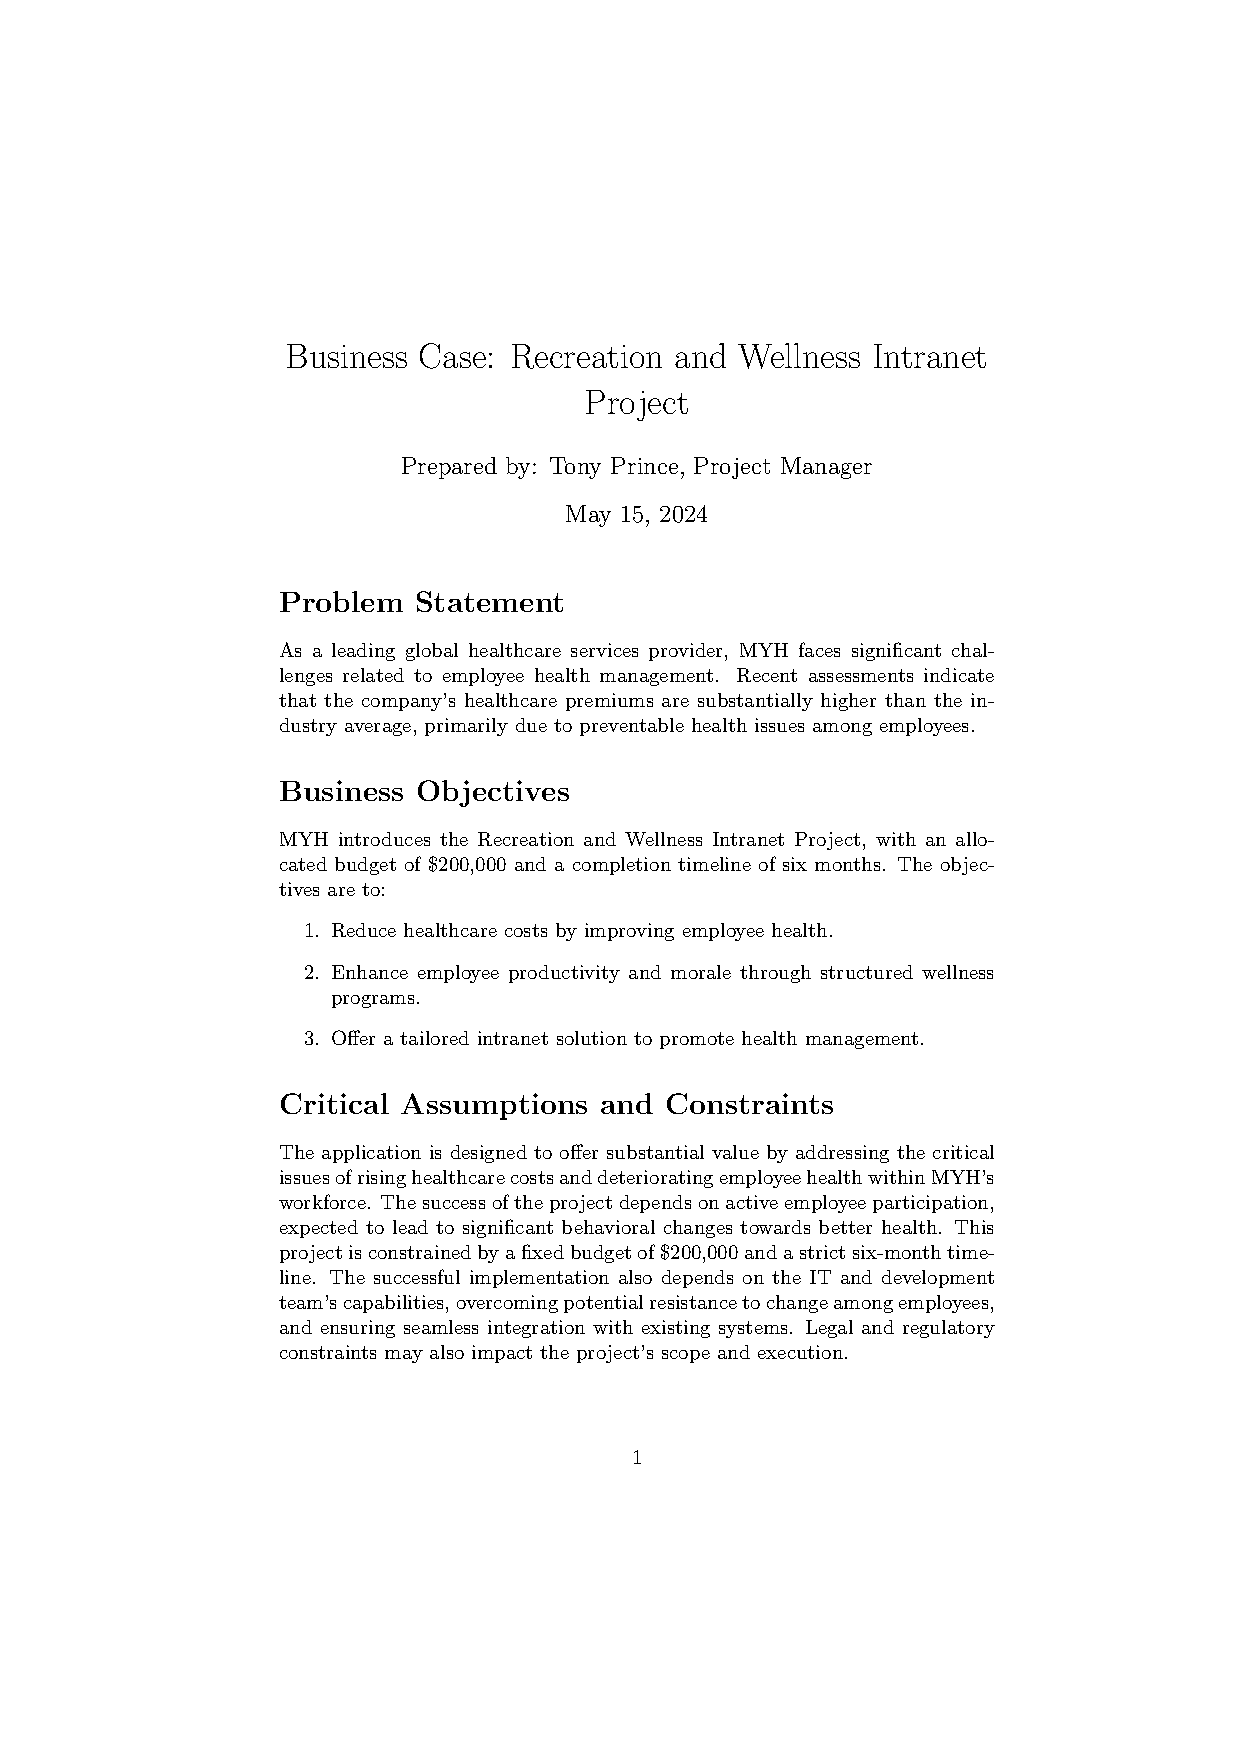
\includepdf[pages=-]{parts/part1/business_case.pdf}

\fancyhead[RO]{\textit{Part2}}
\chapter{Project Scope Management}
Need to be added
\section{Section1}
Need to be added
\section{Section2}
Need to be added

\fancyhead[RO]{\textit{Part3}}
\chapter{Project Schedule Management}
Need to be added
\section{Section1}
Need to be added
\section{Section2}
Need to be added

\fancyhead[RO]{\textit{Part4}}
\chapter{Project Quality Management}
Need to be added
\section{Section1}
Need to be added
\section{Section2}
Need to be added

\fancyhead[RO]{\textit{Part5}}
\chapter{Project Resource Management}
Need to be added
\section{Section1}
Need to be added
\section{Section2}
Need to be added

\FloatBarrier
\newpage

\fancyhead[RO]{\textit{Part6}}
\chapter{Project Risk Management}
\begin{longtable}{|p{1cm}|p{2.5cm}|c|p{1.8cm}|p{1.4cm}|p{1cm}|p{1.8cm}|p{2cm}|}
    \caption{Risk Management Table} \label{tab:title}
    \hline
    \textbf{Risk ID} & \textbf{Risk Description} & \textbf{Type} & \textbf{Probability (1-10)} & \textbf{Impact (1-10)} & \textbf{Risk Score} & \textbf{Response Strategy} & \textbf{Cost Estimate} \\
    \hline
    R1 & Key team members leaving the company & Negative & 8 & 9 & 72 & Mitigate & \$8500 \\
    \hline
    R2 & Uncooperative users & Negative & 7 & 8 & 56 & Mitigate & \$3500 \\
    \hline
    R3 & High employee engagement & Positive & 5 & 9 & 45 & Enhance & \$5000 + \$1000/month \\
    \hline
    R4 & Inability to track data effectively & Negative & 6 & 7 & 42 & Mitigate & \$4000 \\
    \hline
    R5 & Team members not providing good status information & Negative & 6 & 7 & 42 & Mitigate & \$2000 \\
    \hline
    R6 & Successful negotiation of lower health insurance premiums & Positive & 4 & 8 & 32 & Enhance & \$2000 \\
    \hline
\end{longtable}

\section*{Risk Actions}
\begin{longtable}{|p{1cm}|p{5cm}|p{9cm}|}
    \caption{Risk Action Table} \label{tab:title}
    \hline
    \textbf{Risk ID} & \textbf{Risk Description} & \textbf{Action} \\
    \hline
    R1 & Key team members leaving the company & Cross-train the members, update project plan, and implement knowledge transfer as well as team building exercises. \\
    \hline
    R2 & Uncooperative users & Conduct user engagement sessions regularly, gather feedback, and offer training sessions. \\
    \hline
    R3 & High employee engagement & Introduce incentive program, marketing campaign, and adjust program based on feedback. \\
    \hline
    R4 & Inability to track data effectively & Implement a robust data tracking system and provide training on how to use it. \\
    \hline
    R5 & Team members not providing good status information & Implement regular status meetings, develop a reporting template, and provide training on reporting. \\
    \hline
    R6 & Successful negotiation of lower health insurance premiums & Collect and present data on improved health metrics, engage in negotiations with insurance providers. \\
    \hline
\end{longtable}

\pagebreak
\section*{Risk Scores}
\begin{longtable}{|c|c|c|c|}
    \caption{Risk Score Table} \label{tab:title}
    \hline
    \textbf{Risk ID} & \textbf{Probability} & \textbf{Impact} & \textbf{Risk Score} \\
    \hline
    R1 & 8 & 9 & 72 \\
    \hline
    R2 & 7 & 8 & 56 \\
    \hline
    R3 & 5 & 9 & 45 \\
    \hline
    R4 & 6 & 7 & 42 \\
    \hline
    R5 & 6 & 7 & 42 \\
    \hline
    R6 & 4 & 8 & 32 \\
    \hline
\end{longtable}

\section*{Rationale for Risk Scores}

\subsection*{Negative Risk: Key team members leaving the company (R1)}
\begin{itemize}
    \item \textbf{Probability: 8} - Given the history of the project and existing turnover, the probability of team members leaving is the highest. 
    \item \textbf{Impact: 9} - Losing key team members can significantly disrupt project progress, requiring time and resources to onboard new members and carry out missed work.
\end{itemize}

\subsection*{Positive Risk: High employee engagement in the programs leading to improved health (R3)}
\begin{itemize}
    \item \textbf{Probability: 5} - There's a moderate chance of high engagement if the programs are well-promoted and incentivized. 
    \item \textbf{Impact: 9} - If successful, high engagement can lead to significant improvements in employee health, thereby achieving project goals and reducing insurance premiums.
\end{itemize}

\section*{Response Strategies}

\subsection*{Negative Risk: Key team members leaving the company (R1)} 
\begin{outline}
    \1 \textbf{Response Strategy: Mitigate}
        \2 \textbf{Tasks:}
            \3 \textbf{Create a knowledge transfer plan:} Document all critical processes and knowledge. (2 weeks, \$2000)
            \3 \textbf{Cross-train team members:} Ensure multiple team members are knowledgeable about critical tasks. (4 weeks, \$4000)
            \3 \textbf{Develop a succession plan:} Identify potential internal replacements and start preliminary training. (2 weeks, \$1500)
            \3 \textbf{Engage in team-building activities:} Improve team cohesion and job satisfaction. (1 week, \$1000)
\end{outline}
\begin{outline}
    \1 \textbf{Time and Cost Estimates:} 
        \2 Total time: 9 weeks 
        \2 Total cost: \$8500
\end{outline}
\pagebreak
\subsection*{Positive Risk: High employee engagement in the programs leading to improved health (R3)}
\begin{outline}
    \1 \textbf{Response Strategy: Enhance} 
        \2 \textbf{Tasks:}
            \3 \textbf{Develop a marketing campaign:} Create materials to promote the programs. (3 weeks, \$3000)
            \3 \textbf{Introduce incentive programs:} Design rewards for participation and achievements. (2 weeks, \$2000)
            \3 \textbf{Regularly collect and share success stories:} Highlight positive outcomes to motivate others. (Ongoing, \$1000/month)
            \3 \textbf{Monitor and adjust programs:} Continuously improve based on feedback and participation rates. (Ongoing, \$1000/month)
    \1 \textbf{Time and Cost Estimates:} 
        \2 Initial time: 5 weeks 
        \2 Initial cost: \$5000 
        \2 Ongoing cost: \$1000/month

\end{outline}

\FloatBarrier
\newpage

\fancyhead[RO]{\textit{Part7}}
\chapter{Project Stakeholder Management}

This part provides an overview of stakeholder management for this project. Stakeholders are individuals, groups, or organizations that have an interest in the outcome of a project. Managing stakeholders involves identifying who they are, understanding their needs and expectations, and effectively communicating with them throughout the project lifecycle is critical for project success.

\section{Project Team}

The following tables provide detailed information about the project team, including their roles, contact information, and their responsibilities within the project.


    \begin{longtable}{|l|l|l|l|p{6cm}|}
        \caption{Project Team Information} 
        \label{tab:project_team_info} \\
        \hline
        \textbf{Name} & \textbf{Role} & \textbf{Internal/External} & \textbf{Position} \\
        \hline
        \endfirsthead
        \multicolumn{5}{c}%
        {\tablename\ \thetable\ -- \textit{Continued from previous page}} \\
        \hline
        \textbf{Name} & \textbf{Role} & \textbf{Internal/External} & \textbf{Position} \\
        \hline
        \endhead
        \hline \multicolumn{4}{r}{\textit{Continued on next page}} \\
        \endfoot
        \hline
        \endlastfoot
        Tony & Project Manager & Internal & Leader \\
        \hline
        Hillary & Project Sponsor & Internal & Sponsor \\
        \hline
        Karan Goel & Aspiring Project Manager & Internal & Leader \\
        \hline
        Banin Shrestha & Business Analyst & Internal & Team Member \\
        \hline
        Yang & Business Analyst & Internal & Team Member \\
        \hline
        Kushal Rimal & Programmer/Analyst & Internal & Team Member \\
        \hline
        Affan Mehmood & Programmer/Analyst & Internal & Team Member \\
        \hline
        Dipesh Baral & Network Specialist & Internal & Team Member \\
        \hline
        Nora & Network Specialist & Internal & Team Member \\
        \hline
        Ren & Business Analyst & Internal & Team Member \\
        \hline
        Blake & VP of Human Resources & Internal & Sponsor \\
        \hline
        Rose & Human Resource Analyst & Internal & Specialist \\
        \hline
        Tyrian & Financial Analyst & Internal & Specialist \\
        \hline
        Supplier A & System Trainer & External & Supplier \\
        \hline
    \end{longtable}

    \begin{longtable}{|l|l|p{6cm}|}
        \caption{Project Team Contact Information} 
        \label{tab:project_team_contact} \\
        \hline
        \textbf{Name} & \textbf{Email} & \textbf{Contact} \\
        \hline
        \endfirsthead
        \multicolumn{3}{c}%
        {\tablename\ \thetable\ -- \textit{Continued from previous page}} \\
        \hline
        \textbf{Name} & \textbf{Email} & \textbf{Contact} \\
        \hline
        \endhead
        \hline \multicolumn{3}{r}{\textit{Continued on next page}} \\
        \endfoot
        \hline
        \endlastfoot
        Tony & tony@myh.com & Weekly status meetings, email, phone calls \\
        \hline
        Hillary & hillary@myh.com & Weekly status meetings, email, phone calls \\
        \hline
        Karan Goel & karan.goel@myh.com & Weekly status meetings, email, phone calls \\
        \hline
        Banin Shrestha & banin.shrestha@myh.com & Weekly status meetings, email \\
        \hline
        Yang & yang@myh.com & Weekly status meetings, email \\
        \hline
        Kushal Rimal & kushal.rimal@myh.com & Weekly status meetings, email, code reviews \\
        \hline
        Affan Mehmood & affan.mehmood@myh.com & Weekly status meetings, email, code reviews \\
        \hline
        Dipesh Baral & dipesh.baral@myh.com & Weekly status meetings, email \\
        \hline
        Nora & nora@myh.com & Weekly status meetings, email \\
        \hline
        Ren & ren@myh.com & Weekly status meetings, email \\
        \hline
        Blake & blake@myh.com & Monthly status meetings, email, phone calls \\
        \hline
        Rose & rose@myh.com & Email, phone calls \\
        \hline
        Tyrian & tyrian@myh.com & Monthly status meetings, email \\
        \hline
        Supplier A & suppliera@myh.com & Weekly status meetings, email \\
        \hline
    \end{longtable}
    

\section{Project Team Roles and Interests}

The following table details the roles of each team member, their level of authority, and their interests in the project.


\begin{longtable}{|l|l|l|l|}
    \caption{Project Team Roles and Interests} 
    \label{tab:team_roles_interests} \\
    \hline
    \textbf{Name} & \textbf{Project Role} & \textbf{Level of Authority} & \textbf{Interest} \\
    \hline
    \endfirsthead
    \multicolumn{4}{c}%
    {\tablename\ \thetable\ -- \textit{Continued from previous page}} \\
    \hline
    \textbf{Name} & \textbf{Project Role} & \textbf{Level of Authority} & \textbf{Interest} \\
    \hline
    \endhead
    \hline \multicolumn{4}{r}{\textit{Continued on next page}} \\
    \endfoot
    \hline
    \endlastfoot
    Tony & Project Manager & High & Leading \\
    \hline
    Hillary & Project Sponsor & High & Leading \\
    \hline
    Karan Goel & Aspiring Project Manager & High & Leading \\
    \hline
    Banin Shrestha & Business Analyst & Medium & Supportive \\
    \hline
    Yang & Business Analyst & Medium & Supportive \\
    \hline
    Kushal Rimal & Programmer/Analyst & Medium & Supportive \\
    \hline
    Affan Mehmood & Programmer/Analyst & Medium & Supportive \\
    \hline
    Dipesh Baral & Network Specialist & Medium & Supportive \\
    \hline
    Nora & Network Specialist & Medium & Supportive \\
    \hline
    Ren & Business Analyst & Medium & Supportive \\
    \hline
    Blake & VP of Human Resources & High & Leading \\
    \hline
    Rose & Human Resource Analyst & Medium & Supportive \\
    \hline
    Tyrian & Financial Analyst & Medium & Supportive \\
    \hline
    Supplier A & System Trainer & Medium & Supportive \\
    \hline
\end{longtable}

\begin{longtable}{|p{2.3cm}|p{1.6cm}|p{3cm}|p{3cm}|p{4cm}|}
    \caption{Stakeholder Management Information} 
    \label{tab:stakeholder_management} \\
    \hline
    \textbf{Stakeholder} & \textbf{Role} & \textbf{Most Important Goal} & \textbf{How will he/she contribute} & \textbf{Best way to manage} \\
    \hline
    \endfirsthead
    \multicolumn{5}{c}%
    {\tablename\ \thetable\ -- \textit{Continued from previous page}} \\
    \hline
    \textbf{Stakeholder} & \textbf{Role} & \textbf{Most Important Goal} & \textbf{How will he/she contribute} & \textbf{Best way to manage} \\
    \hline
    \endhead
    \hline \multicolumn{5}{r}{\textit{Continued on next page}} \\
    \endfoot
    \hline
    \endlastfoot
    Hillary & Project Sponsor & Ensure that the MYH Recreation and Wellness System meets the needs of the business and its users. & Will provide support and resources to the project team and approve key decisions. & Keep the project sponsor informed of the project's progress and any potential roadblocks. Regularly seek the project sponsor's input and feedback. \\
    \hline
    Gayle & VP of Human Resources & Ensure that the MYH Recreation and Wellness System meets the needs of the human resources department. & Will provide input on the system's requirements and help to promote the system to employees. & Keep Gayle informed of the progress of the project and seek her input on any aspects of the system that may impact the human resources department or its employees. \\
    \hline
    Supplier A & Training and Incentives Provider & Provide training on the MYH Recreation and Wellness System to employees and manage the incentives program. & Will develop and deliver training materials and manage the incentives program. & Work with Supplier A to develop a training plan and incentives program that meets the needs of the project. Regularly communicate with Supplier A to ensure that the training and incentives program are on track. \\
    \hline
    Employees & Full-Time and Part-Time Employees & Use the MYH Recreation and Wellness System to improve their health and well-being. & Will use the system to track their fitness goals, participate in wellness programs, and earn incentives. & Communicate with employees about the benefits of using the system and provide them with support and training. Regularly collect feedback from employees on the system and use it to make improvements. \\
    \hline
\end{longtable}


\FloatBarrier
\newpage

\fancyhead[RO]{\textit{Part8}}
\chapter{Project Closing and Lessons-Learned}
Need to be added
\section{Section1}
Need to be added
\section{Section2}
Need to be added

\fancyhead[RO]{\textit{Part9}}
\chapter{UML Diagrams}
Need to be added yet
\section{Domain Class Diagram}

\begin{figure}[h!t]
    \centering
    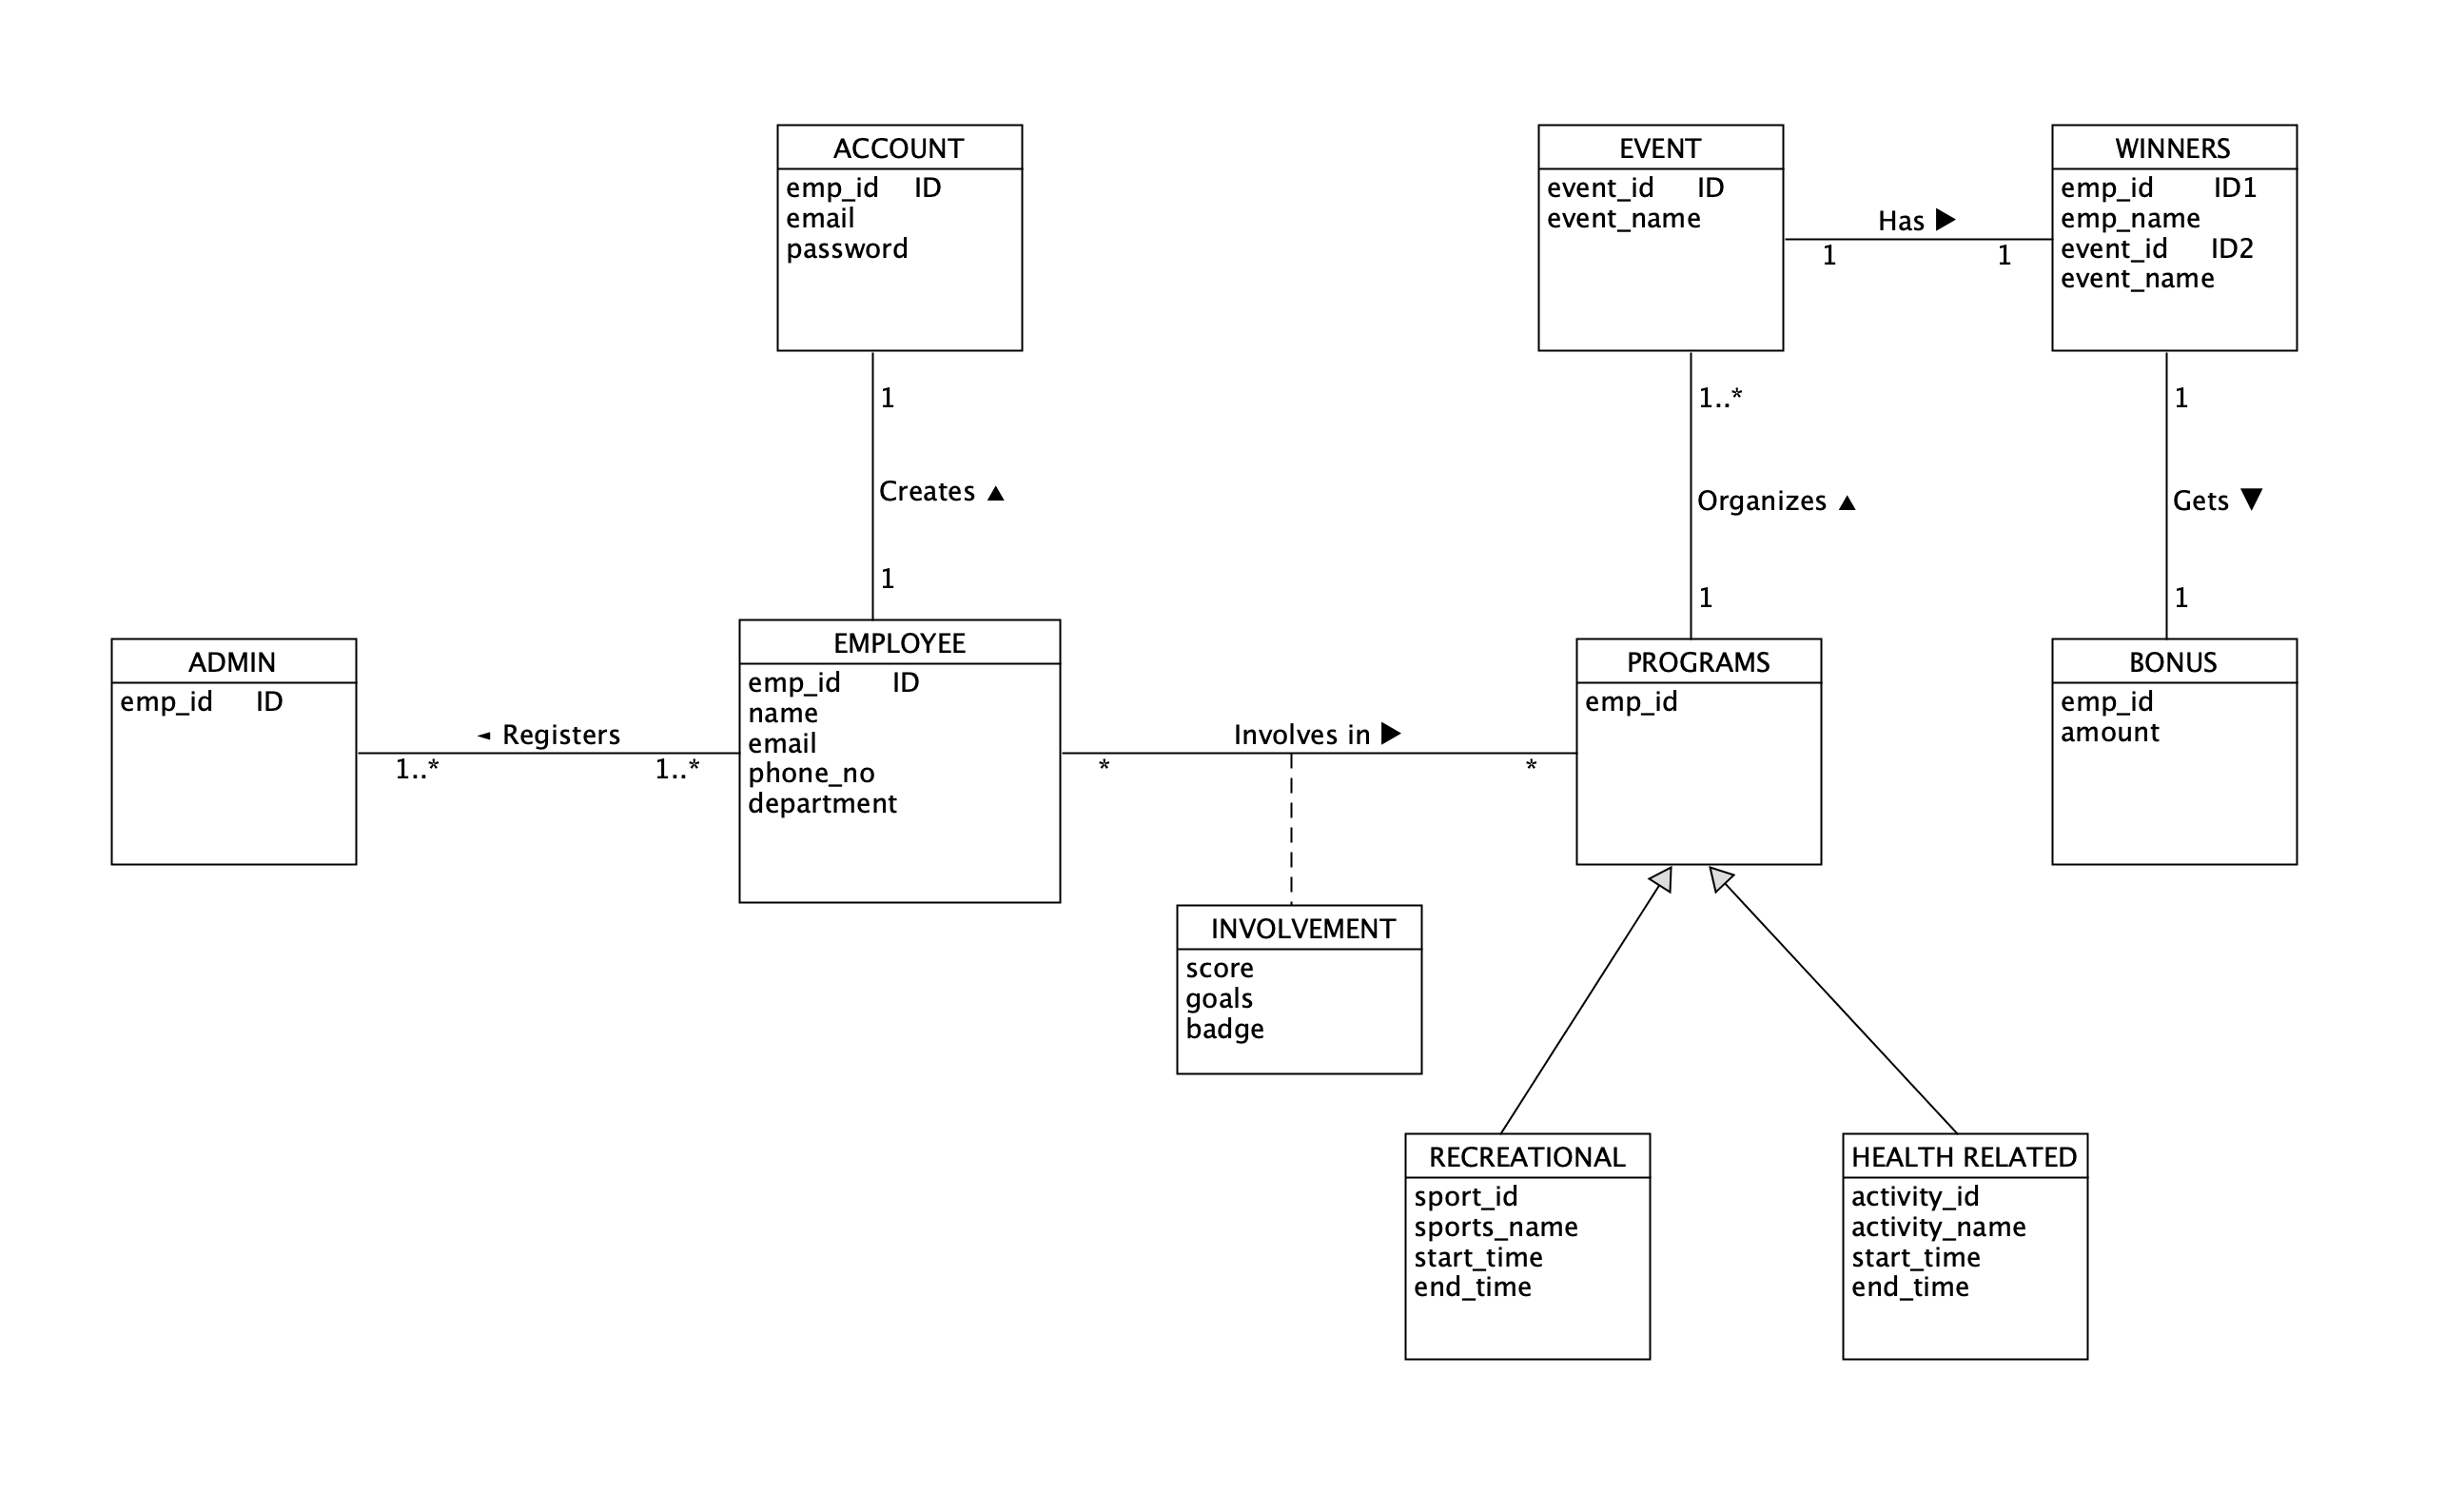
\includegraphics[width=\textwidth]{images/domainClass.png}
    \caption{Domain Class Diagram}
    \label{fig:domainClass}
\end{figure}

\section{Use Case Diagram}


\begin{table}[h!t]
\caption{The Registration Subsystem Use Cases}
{%
\newcommand{\mc}[2]{\multicolumn{#1}{#2}}
\begin{center}
\begin{tabular}{|c|c|}
\hline
\multicolumn{2}{|c|}{\textbf{RWIP Registration Subsystem}} \\ \cline{1-2}
\textbf{Use Cases} & \textbf{Users/Actors} \\
\hline
\rule{0pt}{24pt}  Create Account & Employee \\
\hline
\rule{0pt}{24pt}  Verify Account & Employee \\
\hline
\rule{0pt}{24pt}  Login to Account & Employee \\
\hline
\end{tabular}
\end{center}
}%
\label{tab:reg}
\end{table}

\begin{figure}[h!t]
    \centering
    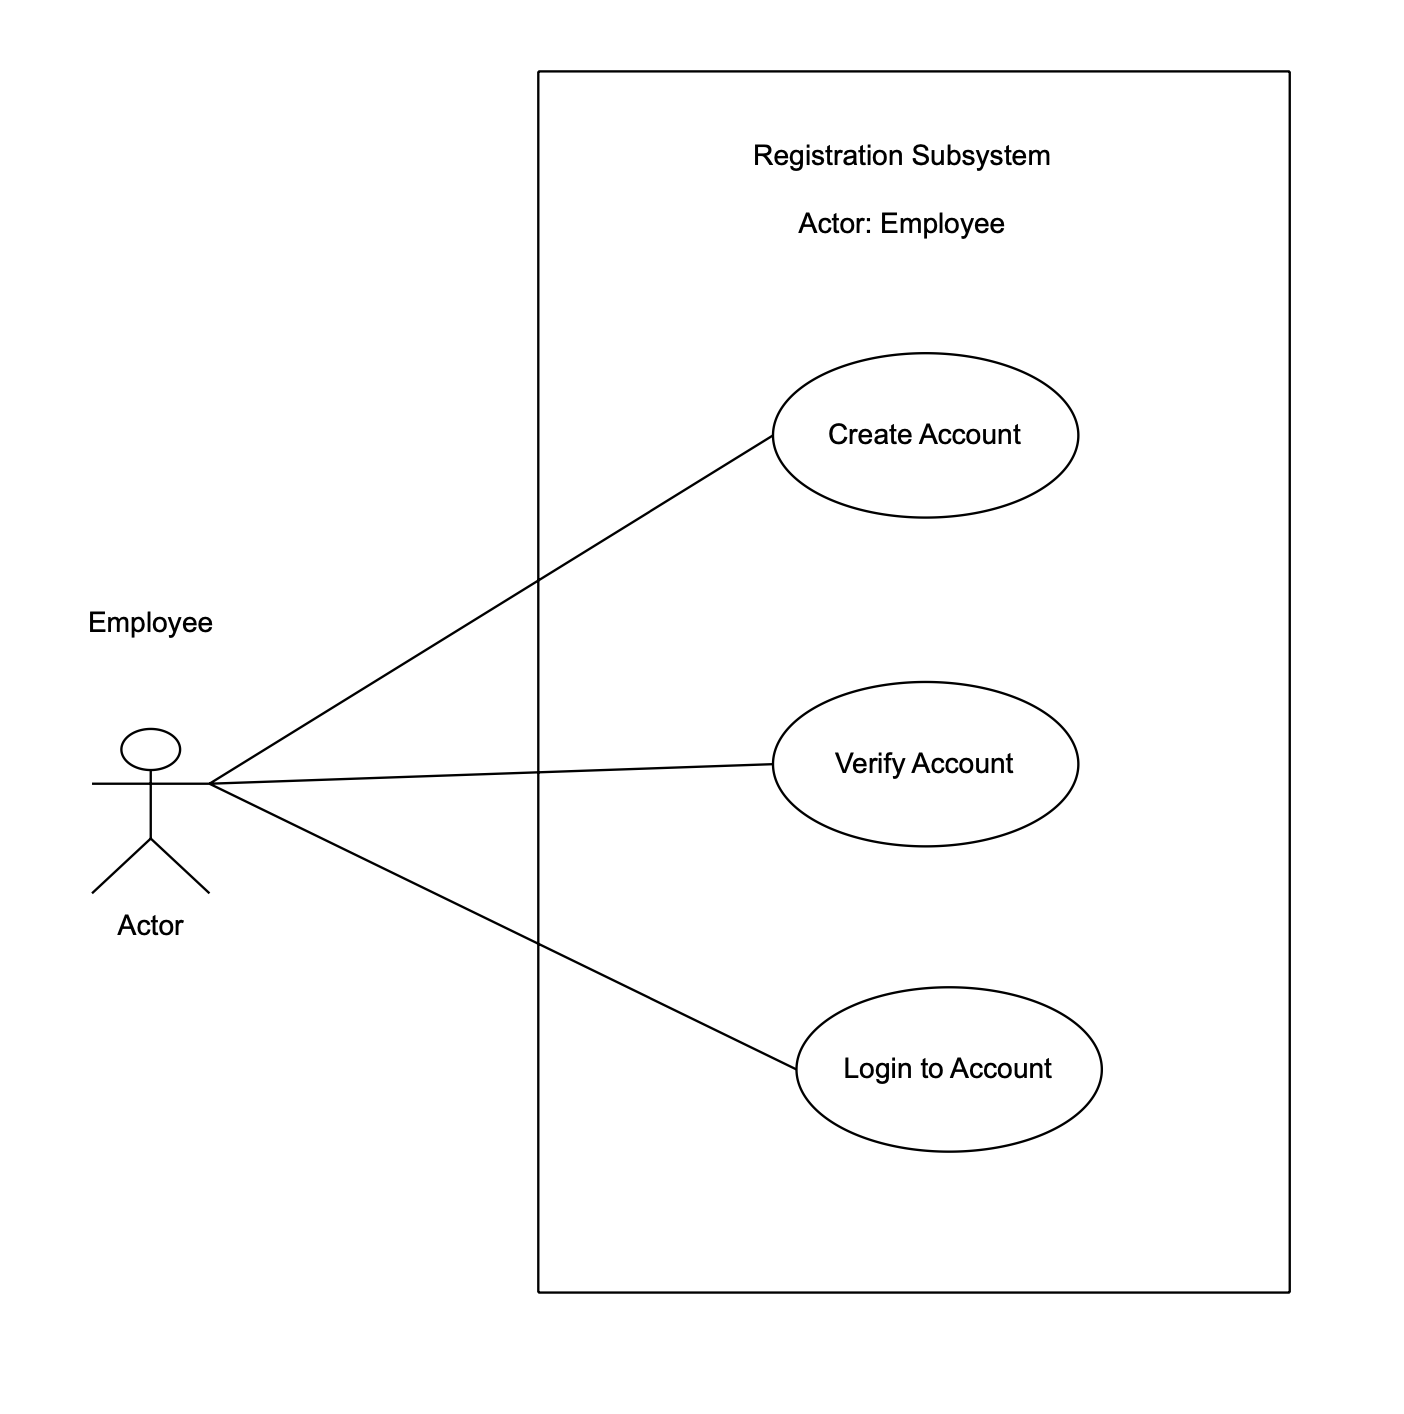
\includegraphics[width=\textwidth]{images/ucRegistration.png}
    \caption{Use case diagram for Registration subsystem}
    \label{fig:ucRegistration}
\end{figure}

\begin{table}[h!t]
\caption{The Program Subsystem Use Cases}
{%
\newcommand{\mc}[2]{\multicolumn{#1}{#2}}
\begin{center}
\begin{tabular}{|c|c|}
\hline
\multicolumn{2}{|c|}{\textbf{RWIP Program Subsystem}} \\ \cline{1-2}
\textbf{Use Cases} & \textbf{Users/Actors} \\
\hline
\rule{0pt}{24pt}  Login & Employee \\
\hline
\rule{0pt}{24pt}  Select Programs & Employee \\
\hline
\rule{0pt}{24pt}  Book/Enroll Programs & Employee \\
\hline
\rule{0pt}{24pt}  Participate in Programs & Employee \\
\hline
\rule{0pt}{24pt}  Update badges and rewards & Employee \\
\hline
\end{tabular}
\end{center}
}%
\label{tab:program}
\end{table}

\begin{figure}[h!t]
    \centering
    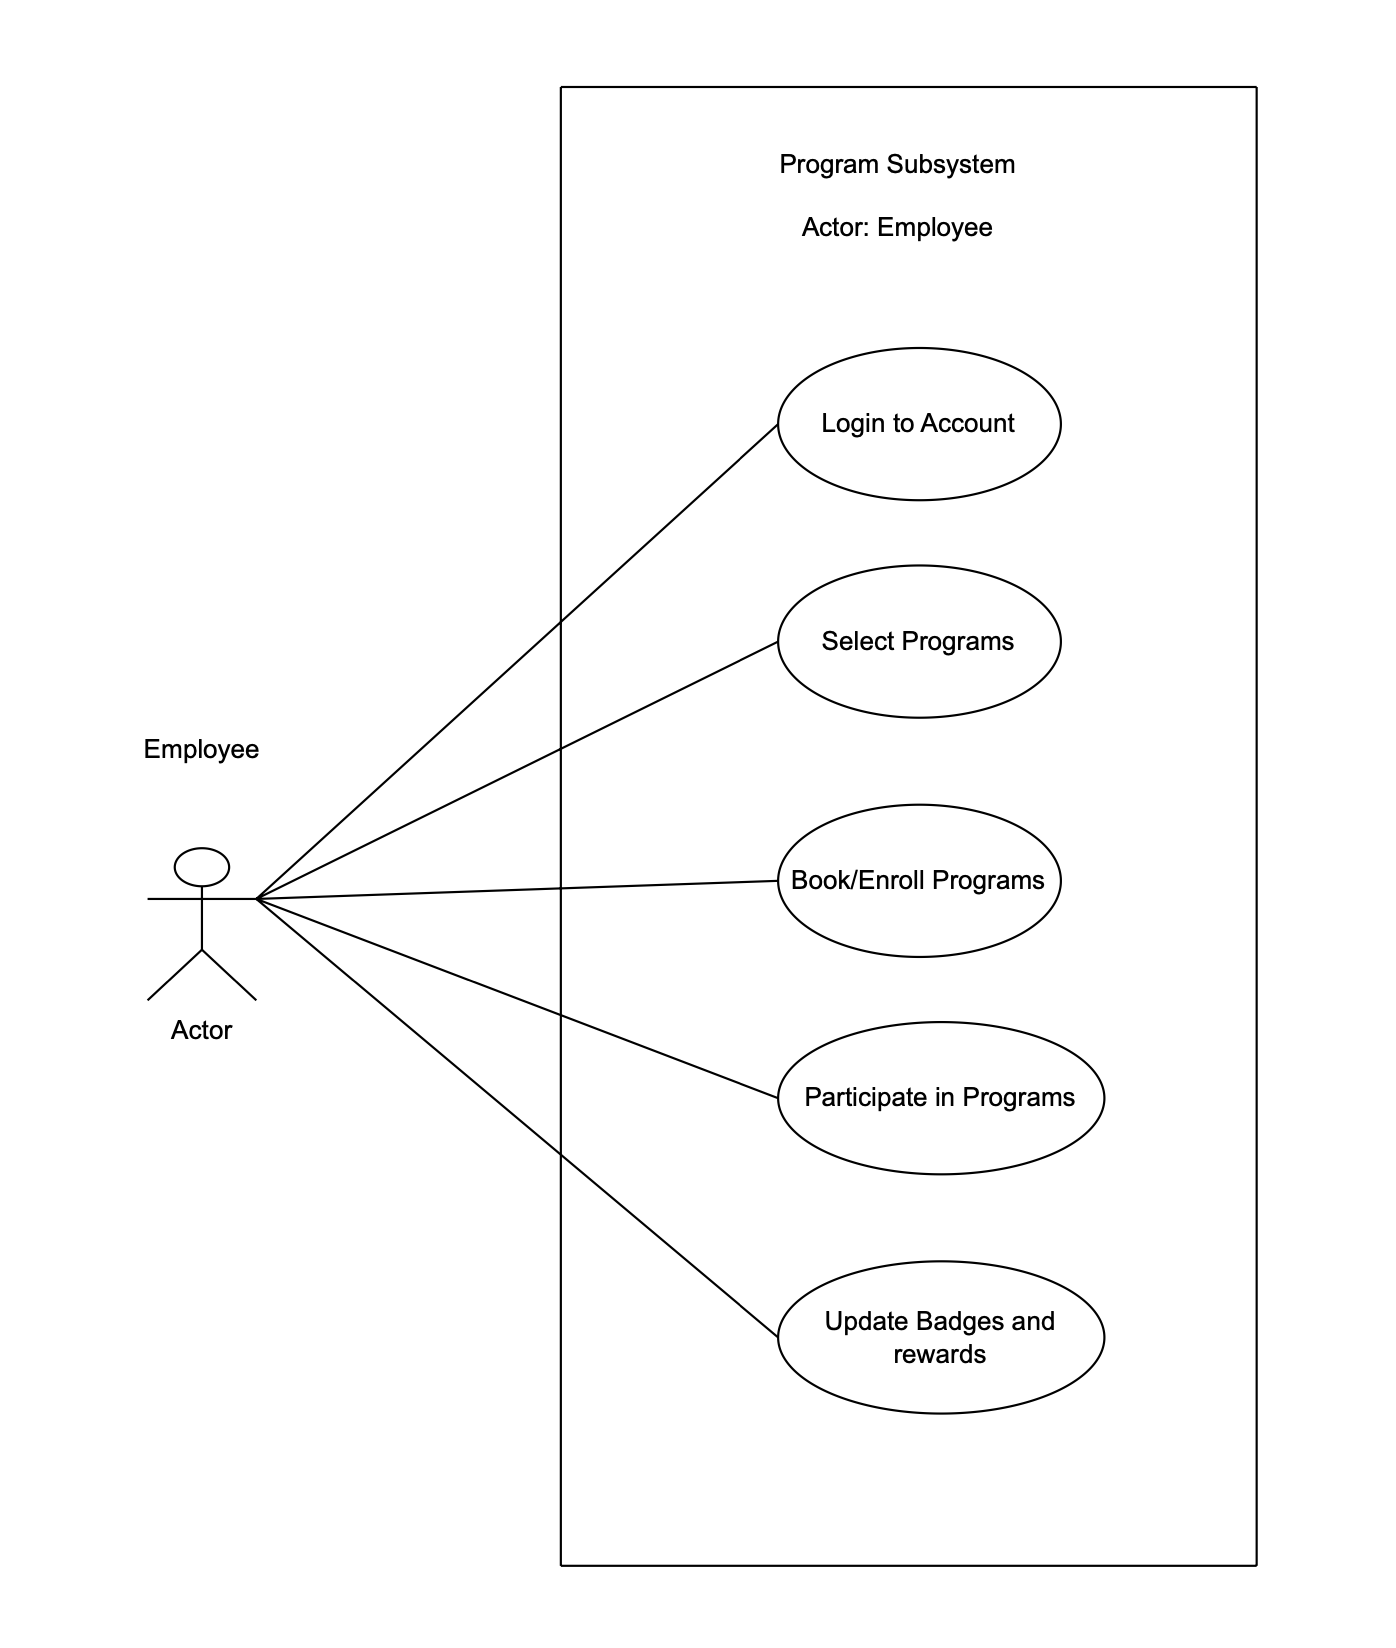
\includegraphics[width=\textwidth]{images/ucProgram.png}
    \caption{Use case diagram for Program subsystem}
    \label{fig:ucProgram}
\end{figure}


\begin{table}[h!t]
\caption{The Event Subsystem Use Cases}
{%
\newcommand{\mc}[2]{\multicolumn{#1}{#2}}
\begin{center}
\begin{tabular}{|c|c|}
\hline
\multicolumn{2}{|c|}{\textbf{RWIP Event Subsystem}} \\ \cline{1-2}
\textbf{Use Cases} & \textbf{Users/Actors} \\
\hline
\rule{0pt}{24pt}  Organise Events & HR/Admin \\
\hline
\rule{0pt}{24pt}  Notify Events & HR/Admin, Employee \\
\hline
\rule{0pt}{24pt}  Design Banner & HR/Admin \\
\hline
\rule{0pt}{24pt}  Participate in Events & Employee \\
\hline
\rule{0pt}{24pt}  Declare winners & HR/Admin, Employee \\
\hline
\end{tabular}
\end{center}
}%
\label{tab:event}
\end{table}

\begin{figure}[h!t]
    \centering
    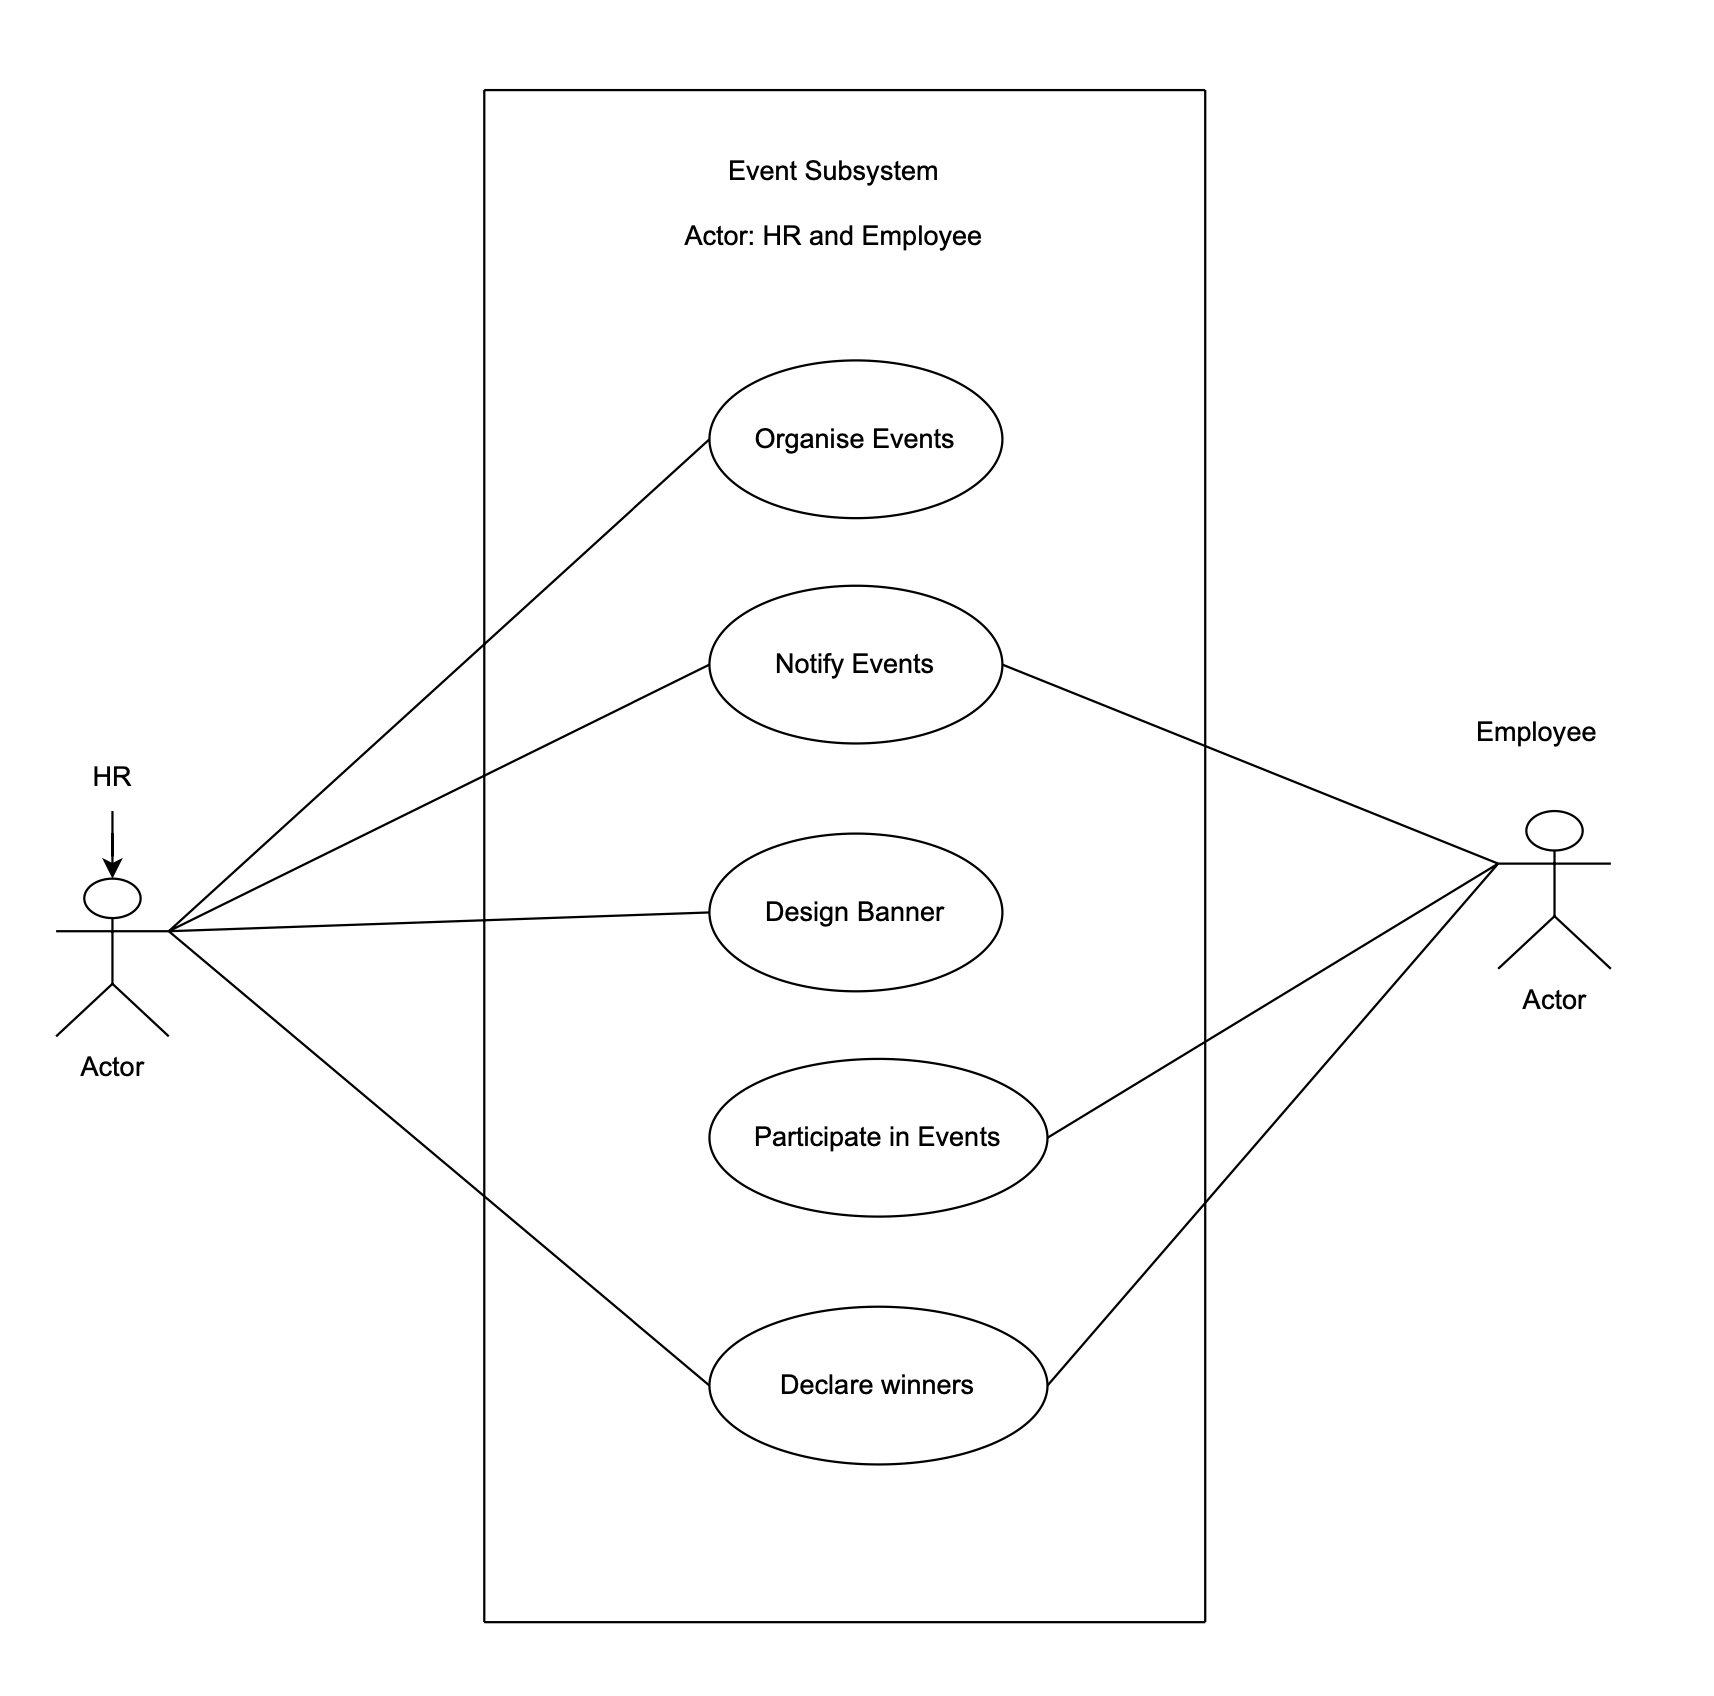
\includegraphics[width=\textwidth]{images/ucEvent.png}
    \caption{Use case diagram for Event subsystem}
    \label{fig:ucEvent}
\end{figure}

\begin{table}[h!t]
\caption{The Payroll Subsystem Use Cases}
{%
\newcommand{\mc}[2]{\multicolumn{#1}{#2}}
\begin{center}
\begin{tabular}{|c|c|}
\hline
\multicolumn{2}{|c|}{\textbf{RWIP Payroll Subsystem}} \\ \cline{1-2}
\textbf{Use Cases} & \textbf{Users/Actors} \\
\hline
\rule{0pt}{24pt} Get the list of winners in different Programs & Payroll Officer, Employee\\
\hline
\rule{0pt}{24pt}  Provide bonuses & Payroll Officer, Employee \\
\hline
\rule{0pt}{24pt}  Update Payroll & Payroll Officer \\
\hline
\end{tabular}
\end{center}
}%
\label{tab:payroll}
\end{table}

\begin{figure}[h!t]
    \centering
    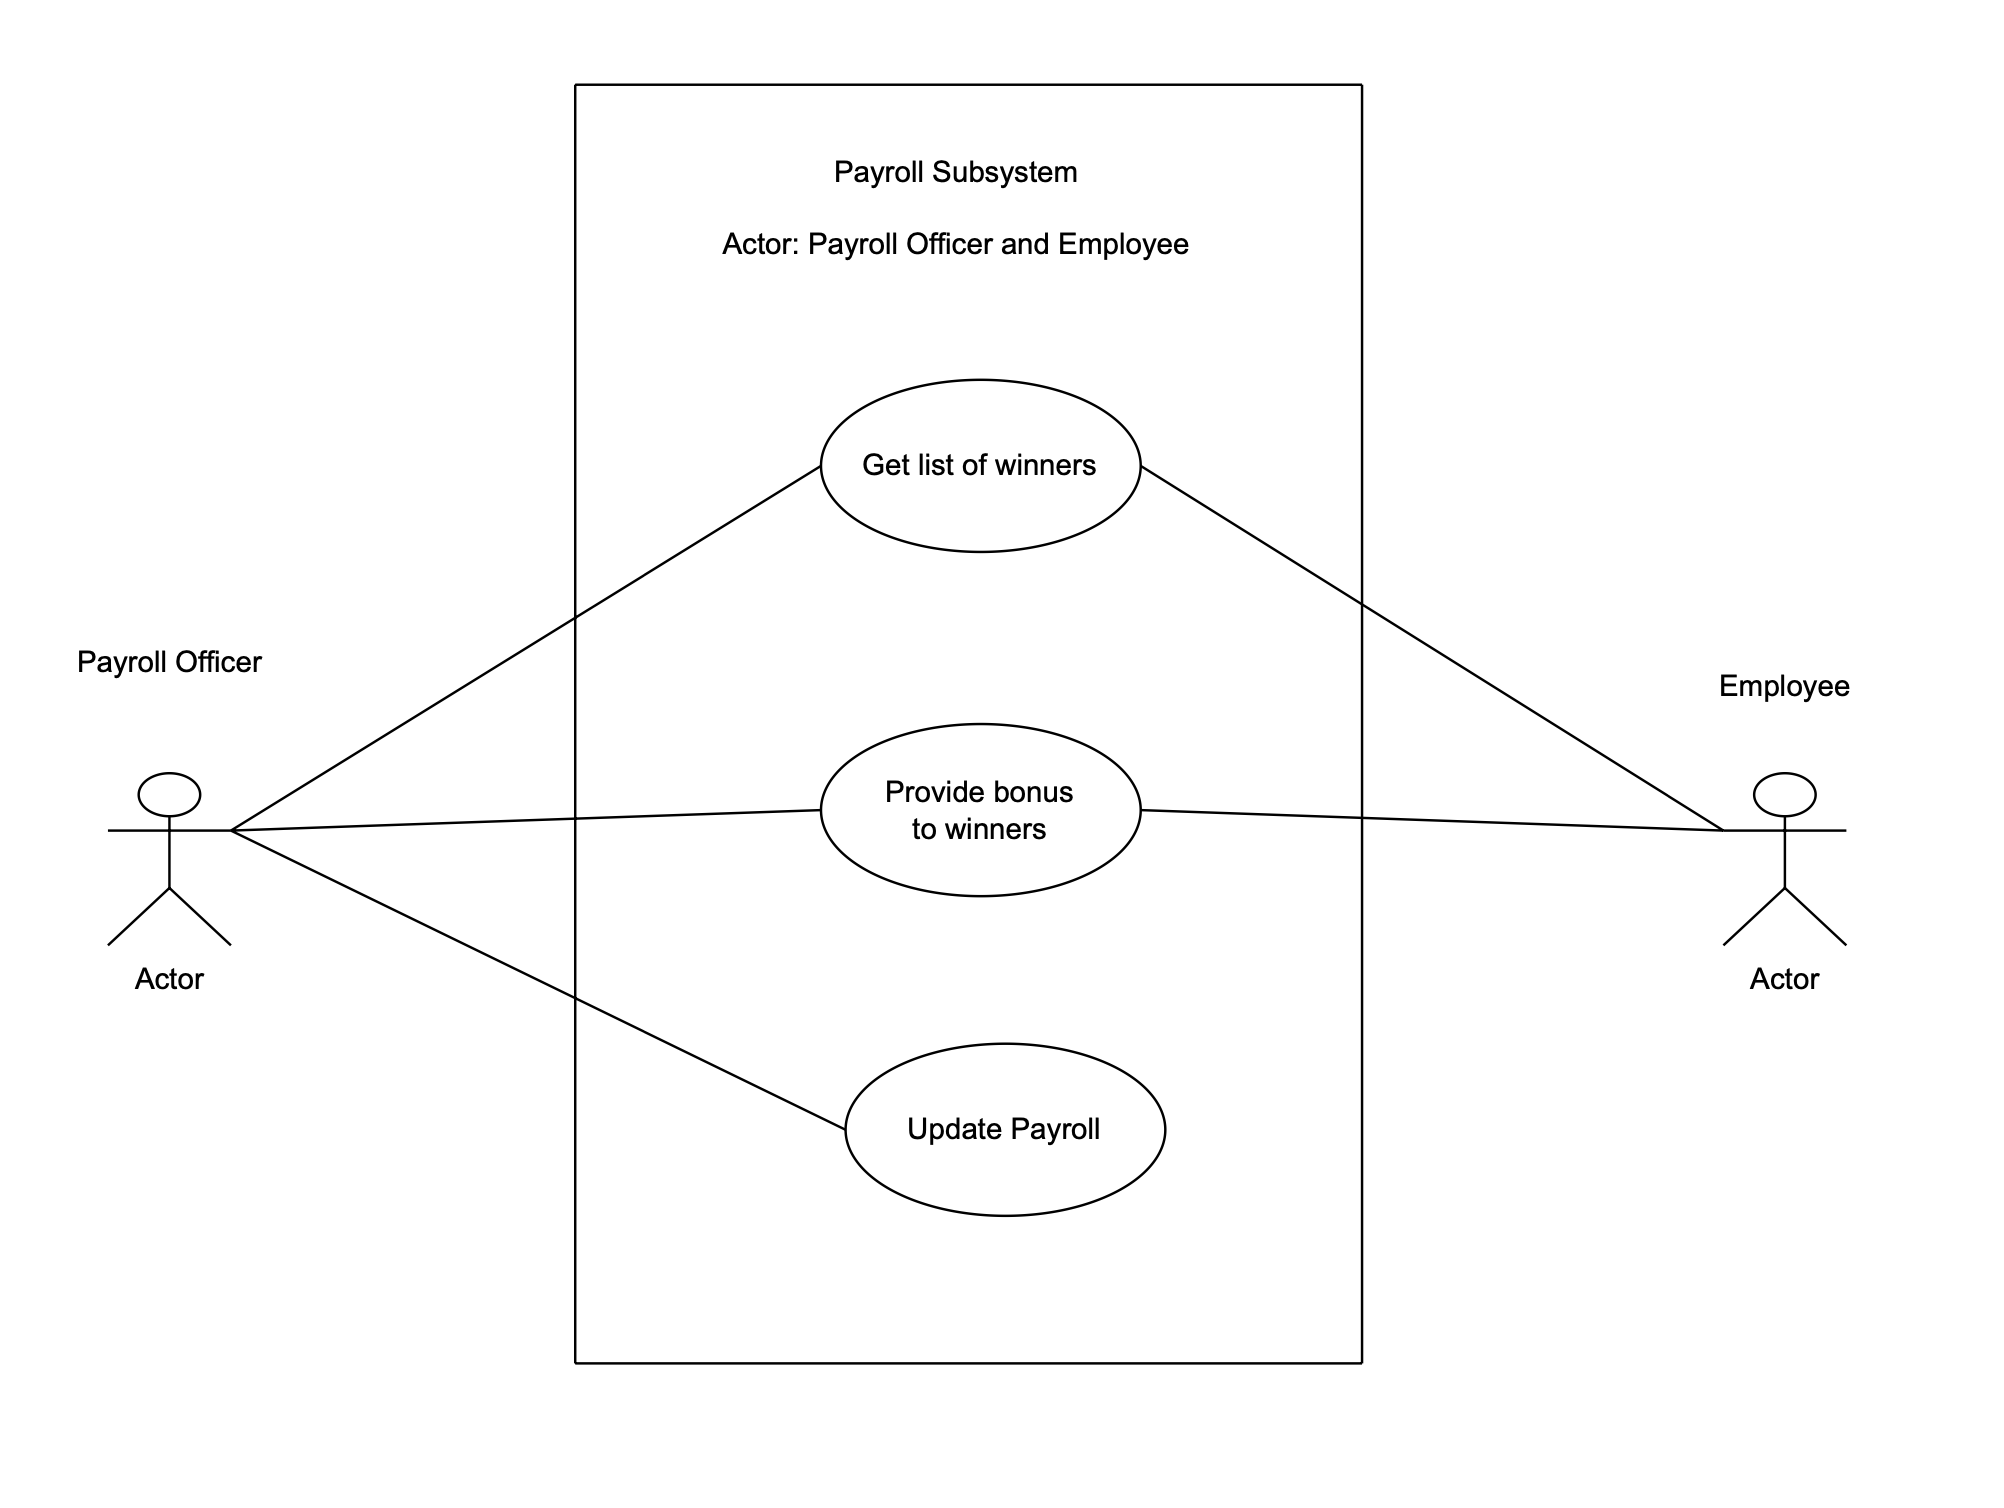
\includegraphics[width=\textwidth]{images/ucPayroll.png}
    \caption{Use case diagram for Payroll subsystem}
    \label{fig:ucPayroll}
\end{figure}

\begin{table}[h!t]
\caption{The Analysis Subsystem Use Cases}
{%
\newcommand{\mc}[2]{\multicolumn{#1}{#2}}
\begin{center}
\begin{tabular}{|c|c|}
\hline
\multicolumn{2}{|c|}{\textbf{RWIP Analysis Subsystem}} \\ \cline{1-2}
\textbf{Use Cases} & \textbf{Users/Actors} \\
\hline
\rule{0pt}{24pt}  Register as Admin & Analyst \\
\hline
\rule{0pt}{24pt}  Login as Admin & Analyst \\
\hline
\rule{0pt}{24pt}  Fetch Data & Analyst \\
\hline
\rule{0pt}{24pt}  Analyze Data & Analyst \\
\hline
\rule{0pt}{24pt}  Generate Report & Analyst, Developers \\
\hline
\rule{0pt}{24pt}  Make Decisions & Analyst \\
\hline
\end{tabular}
\end{center}
}%
\label{tab:analysis}
\end{table}

\begin{figure}[h!t]
    \centering
    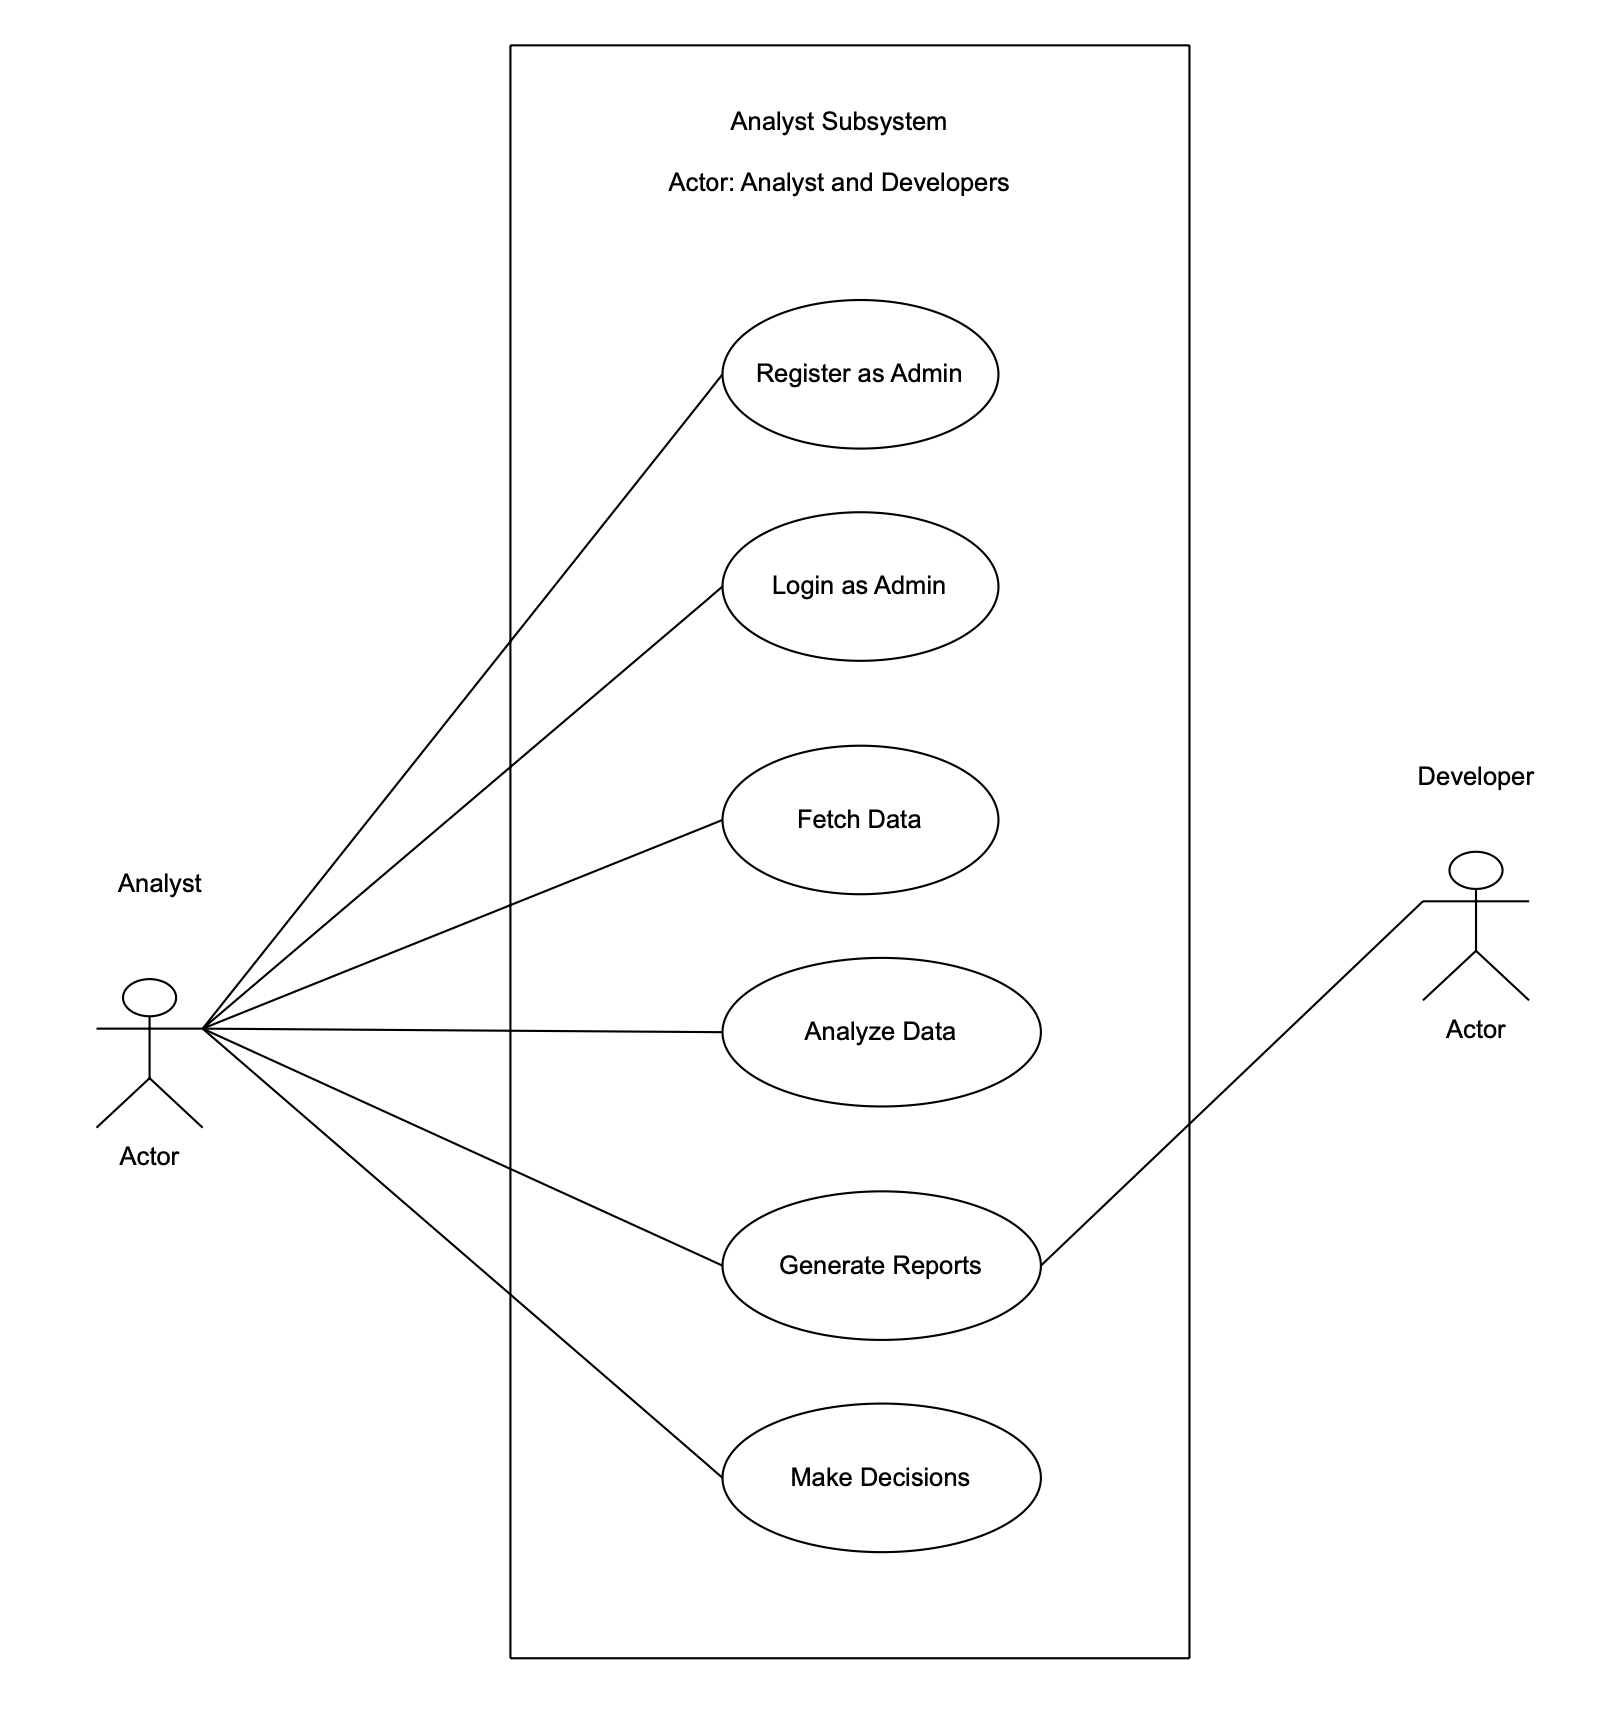
\includegraphics[width=\textwidth]{images/ucAnaysis.png}
    \caption{Use case diagram for Analysis subsystem}
    \label{fig:ucAnaysis}
\end{figure}


\section{Fully Developed Use Case Description}

\begin{table}[h!t]
\caption{Register/Create Account}

\begin{center}
\begin{tabular}{|c|c|}
\hline

\rule{0pt}{24pt}  \textbf{Use case name:} & Create employee account \\
\hline
\rule{0pt}{24pt}  \textbf{Scenario:} & Create online employee account \\
\hline
\rule{0pt}{24pt}  \textbf{Triggering event:} & Employee wants to join the recreational and wellness programs \\
\hline
\rule{0pt}{24pt}  \textbf{Brief description:} & Employee signs up or creates new account by providing their employee email id to access, book and participate in activity \\
\hline
\rule{0pt}{24pt}  \textbf{Actors:} & Employees \\
\hline
\rule{0pt}{24pt}  \textbf{Related use cases:} & Admin can create account on behalf of employee \\
\hline
\rule{0pt}{24pt}  \textbf{Stakeholders:} & Admin, HR \\
\hline
\rule{0pt}{24pt}  \textbf{Pre-conditions:} & Registration subsystem must be available \\
% Employees must have employer's provided email_id \\
% Employees must verify the account by clicking on verify link sent on the email
\hline
\rule{0pt}{24pt}  \textbf{Post-conditions:} & Employee account must be created and saved \\
% All the activity must be tracked like badge, rewards received.
\hline
\rule{0pt}{24pt}  \textbf{Exception conditions:} & Employee might not have email id provided by employer \\
% Employee have not verified the account by clicking on verification link sent on the mail.
% Email_id provided is invalid
\hline
\end{tabular}
\end{center}
\label{tab:createAccount}
\end{table}


\section{Sequence Diagram}

\begin{figure}[h!t]
    \centering
    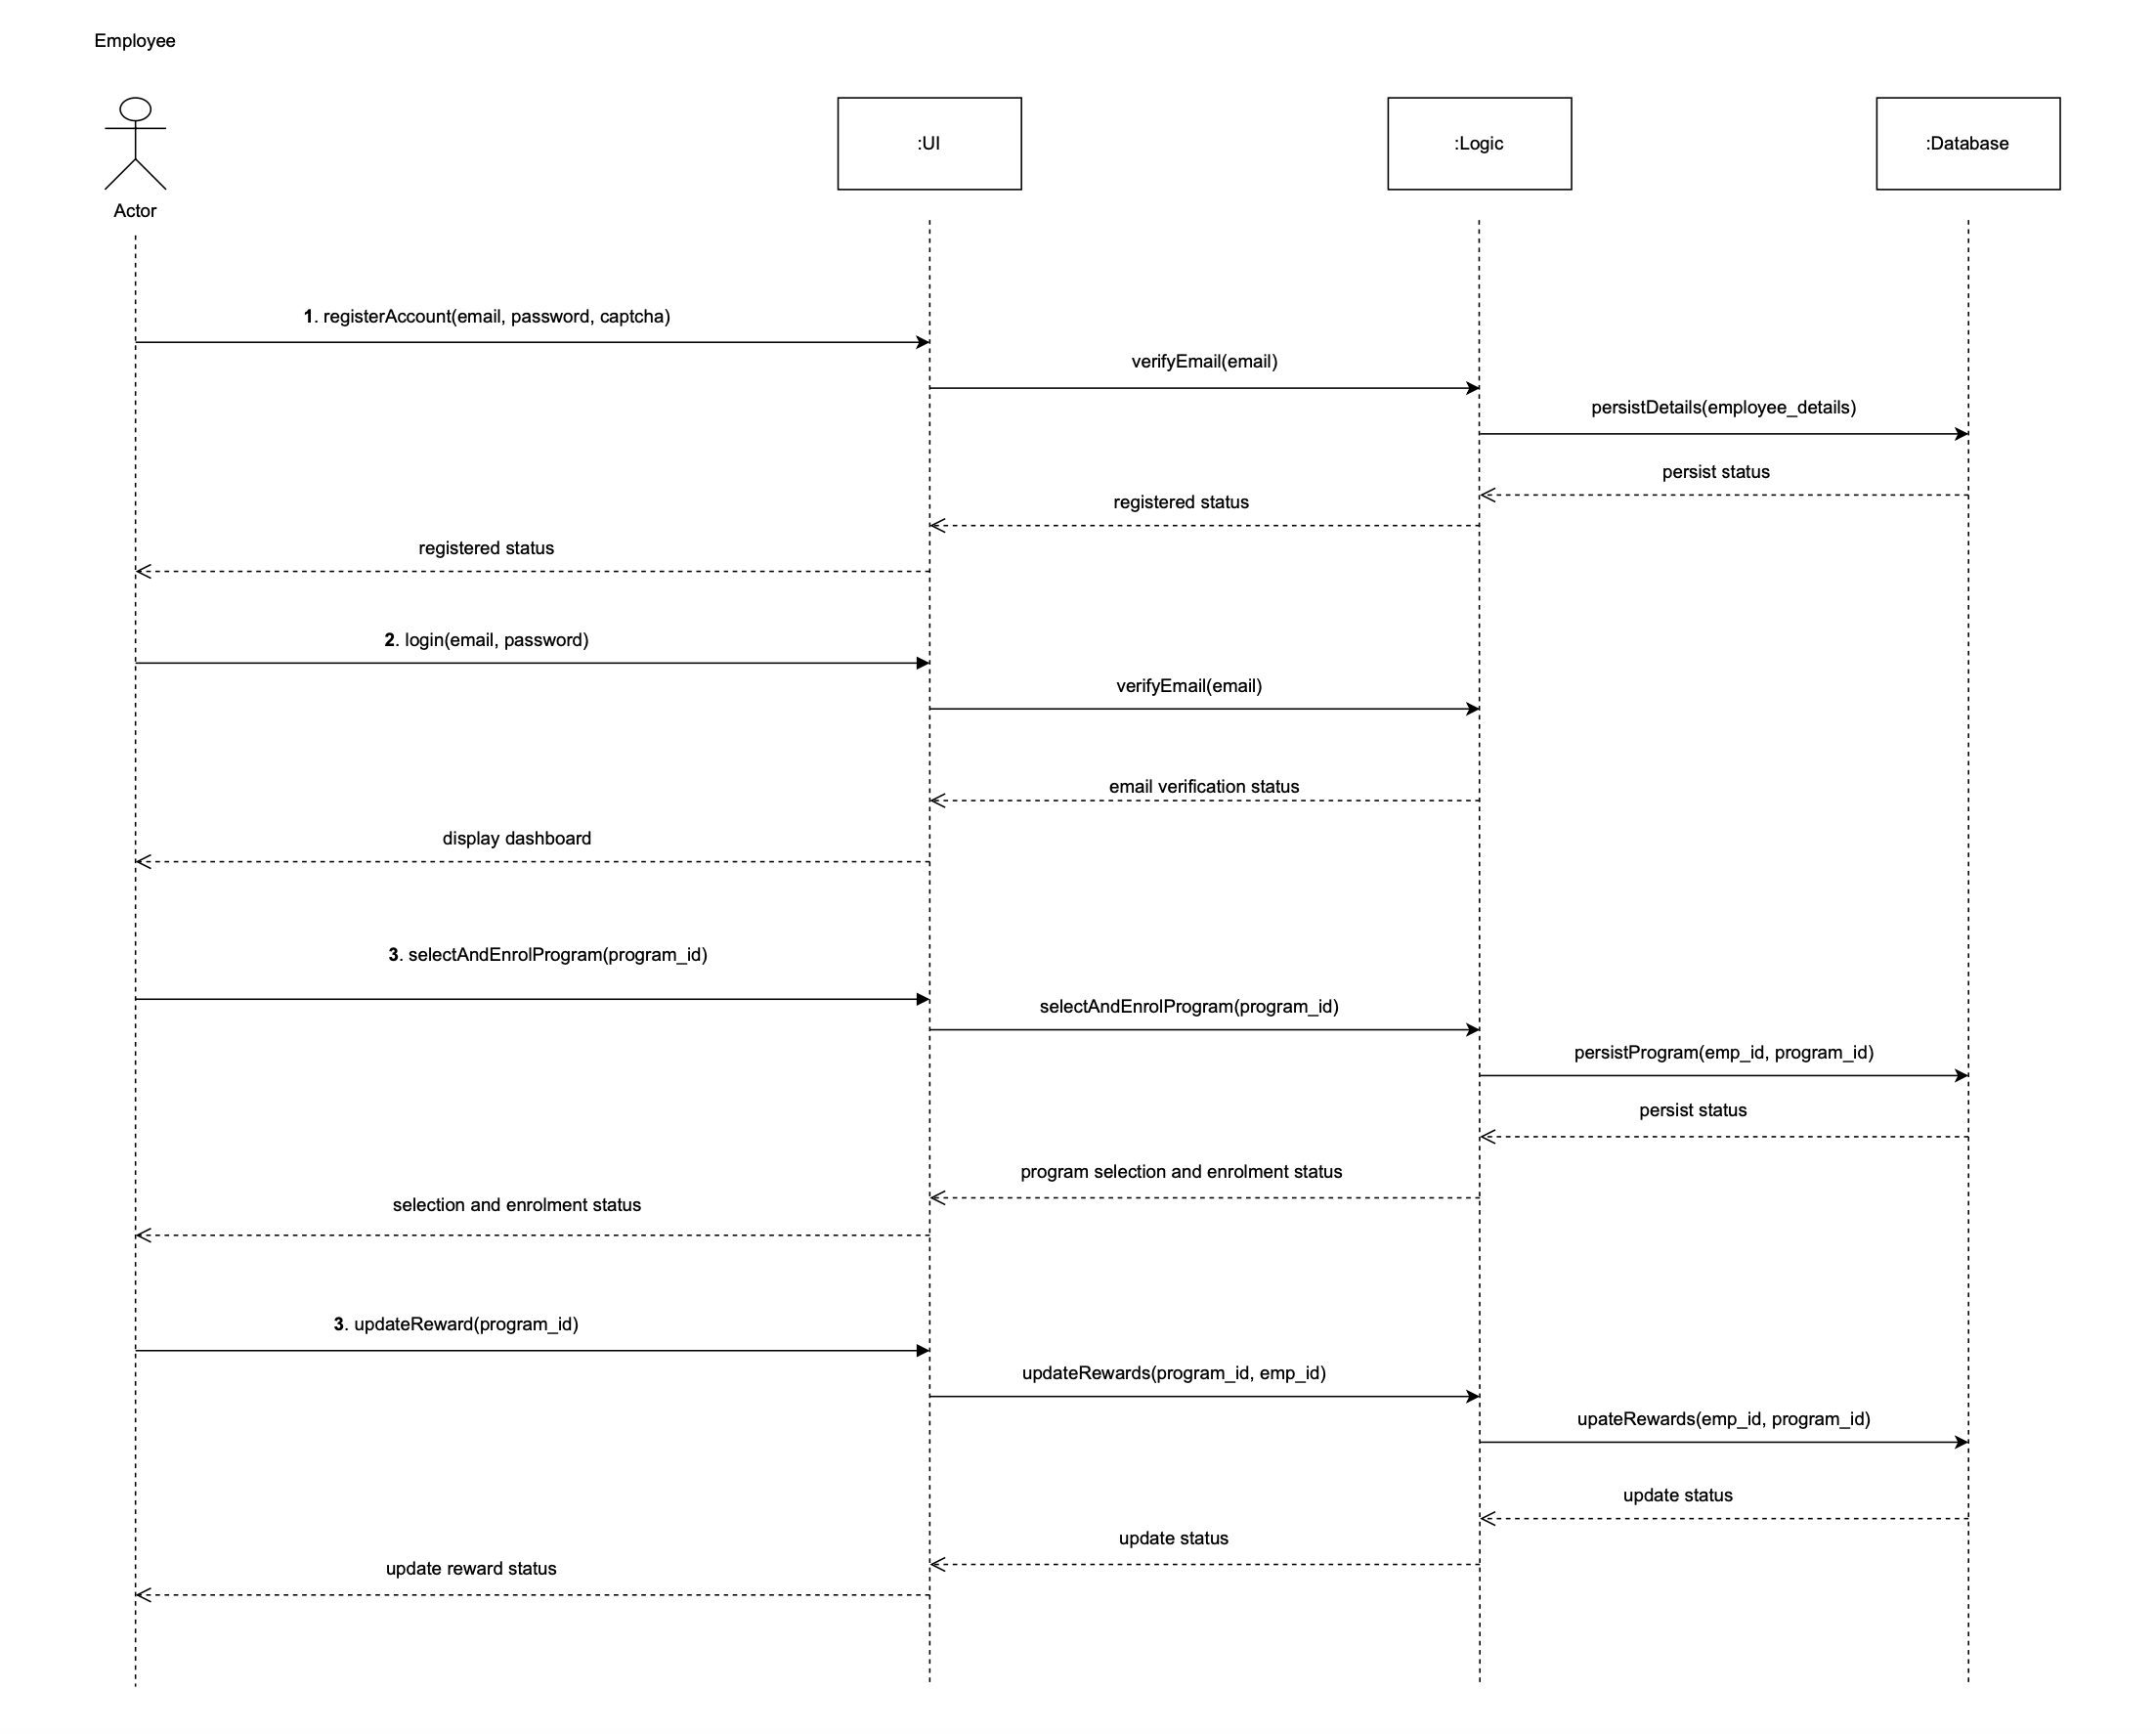
\includegraphics[width=\textwidth]{images/sequenceDiagram.png}
    \caption{Activity Diagram of all the subsystem}
    \label{fig:sequenceDiagram}
\end{figure}


\section{Activity Diagram}

\begin{figure}[h!t]
    \centering
    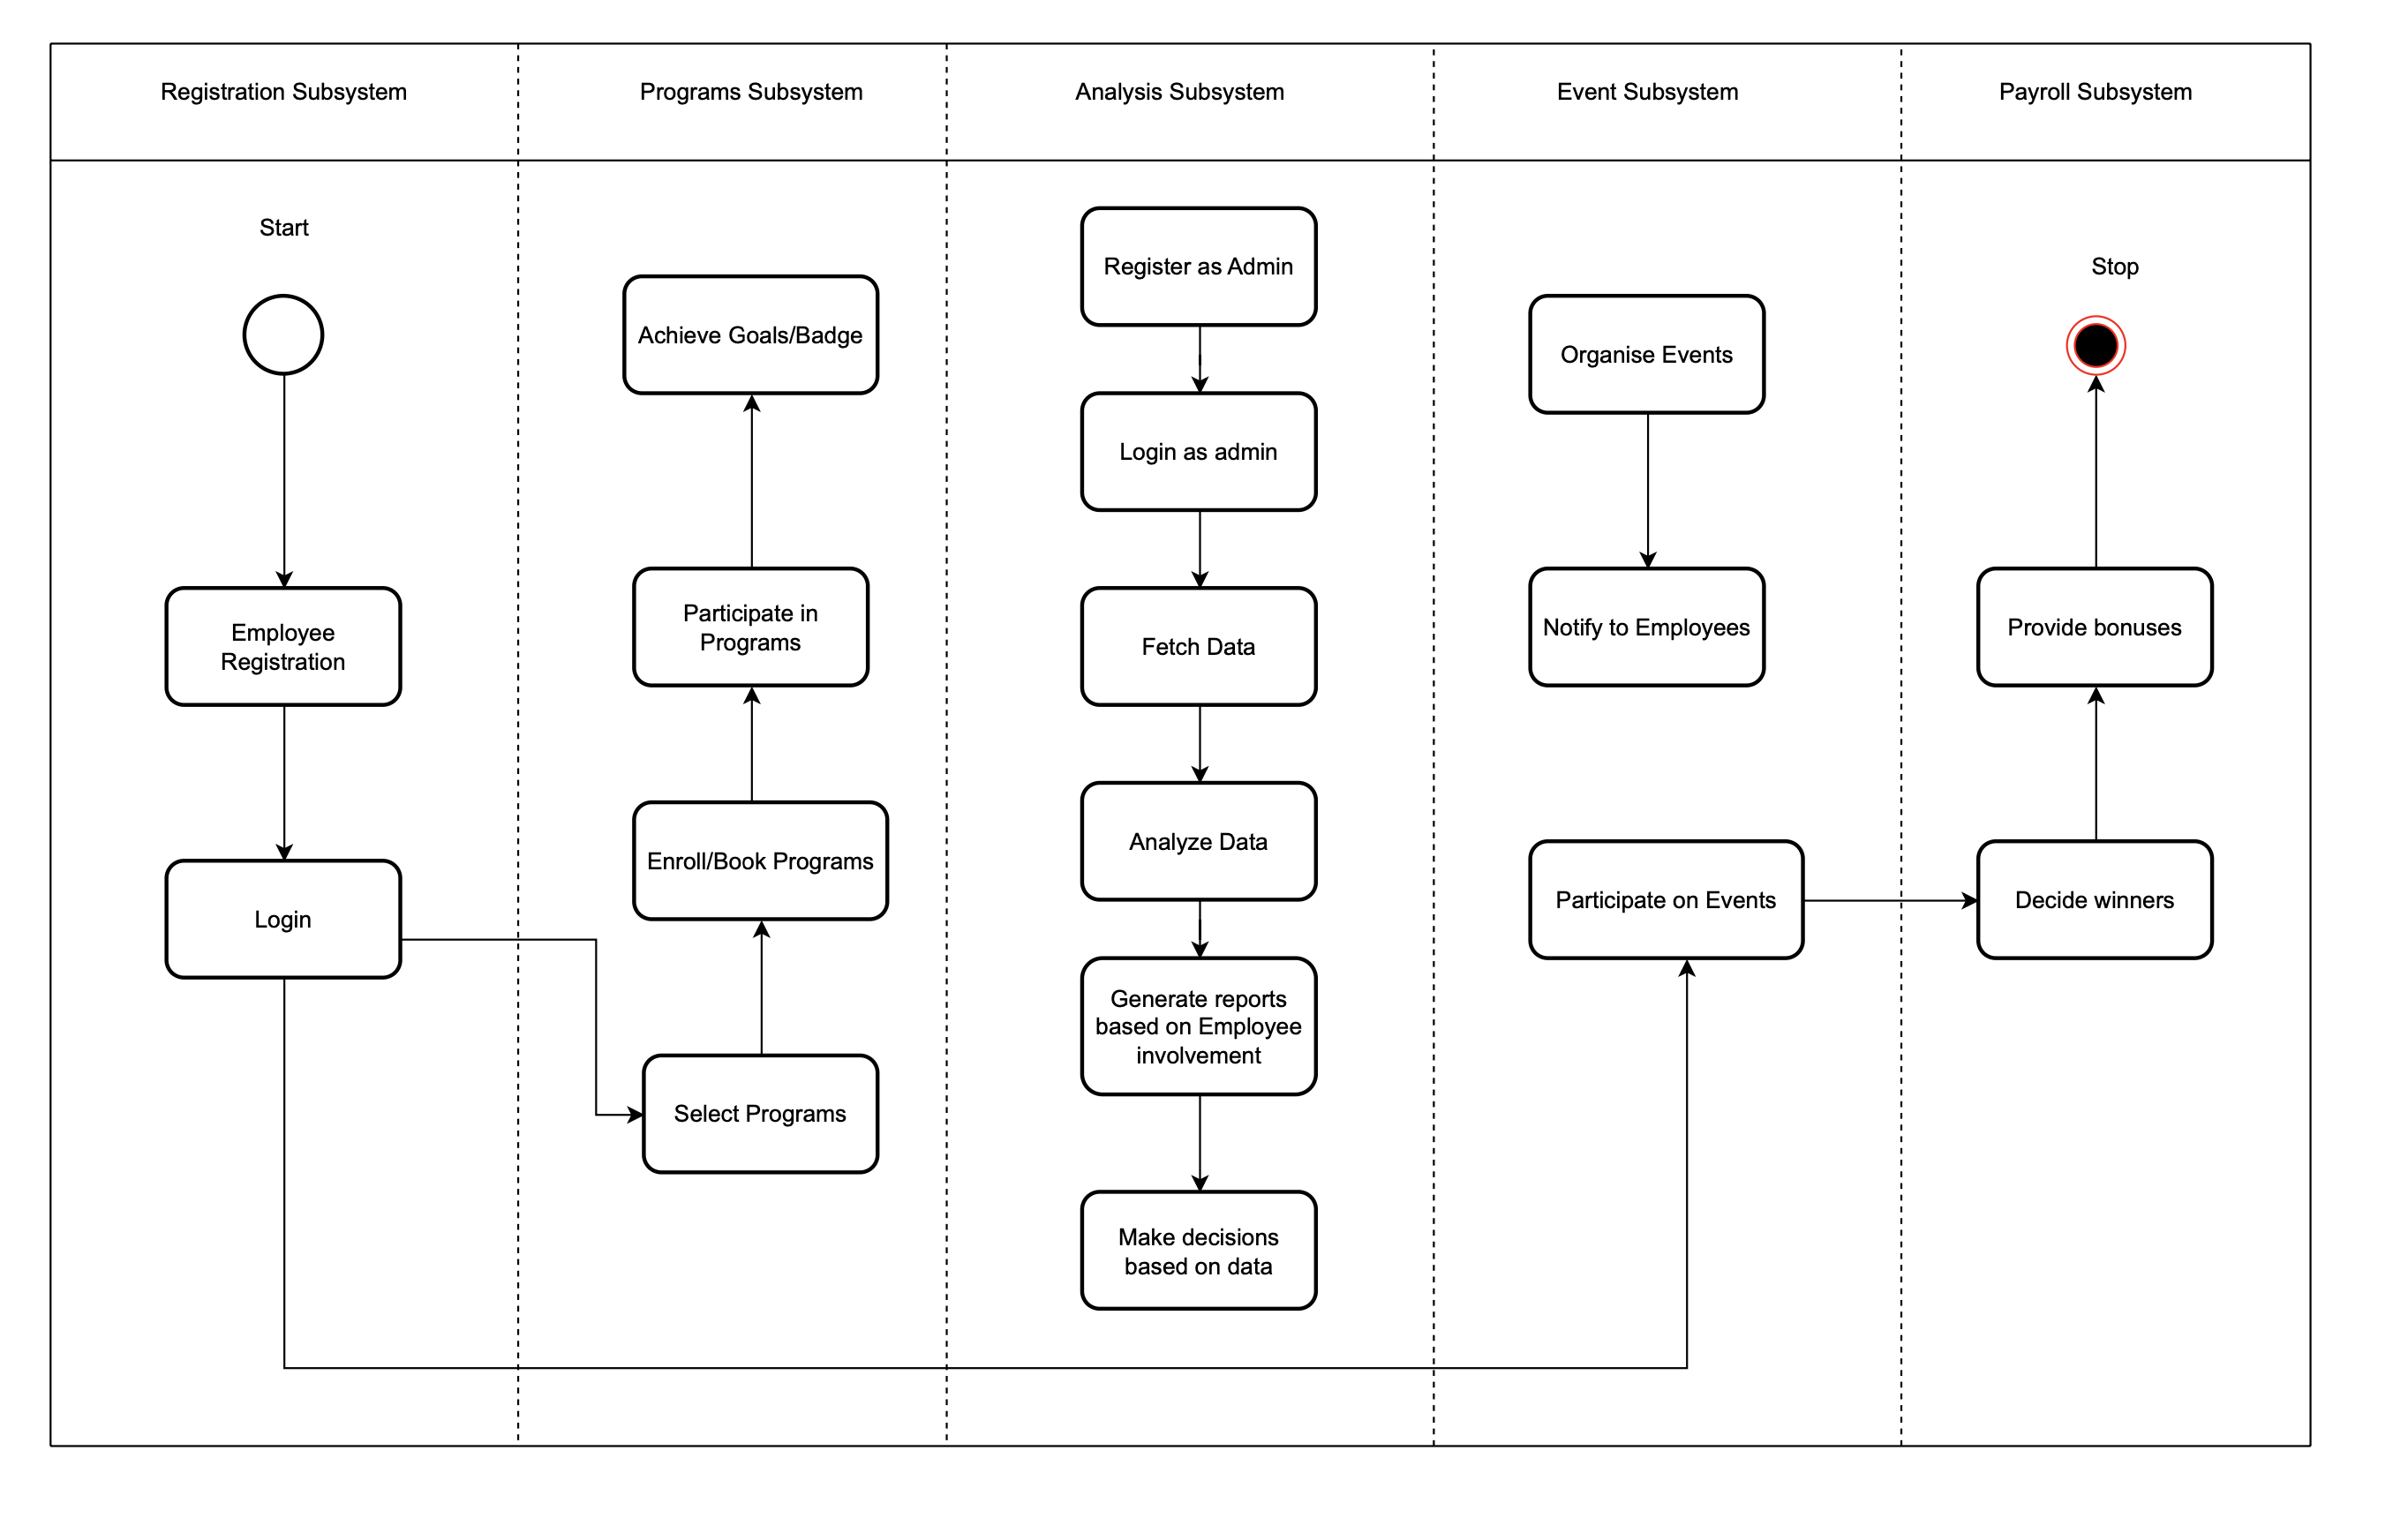
\includegraphics[width=\textwidth]{images/activityDiagram.png}
    \caption{Activity Diagram of all the subsystem}
    \label{fig:activityDiagram}
\end{figure}

\begin{figure}[h!t]
    \centering
    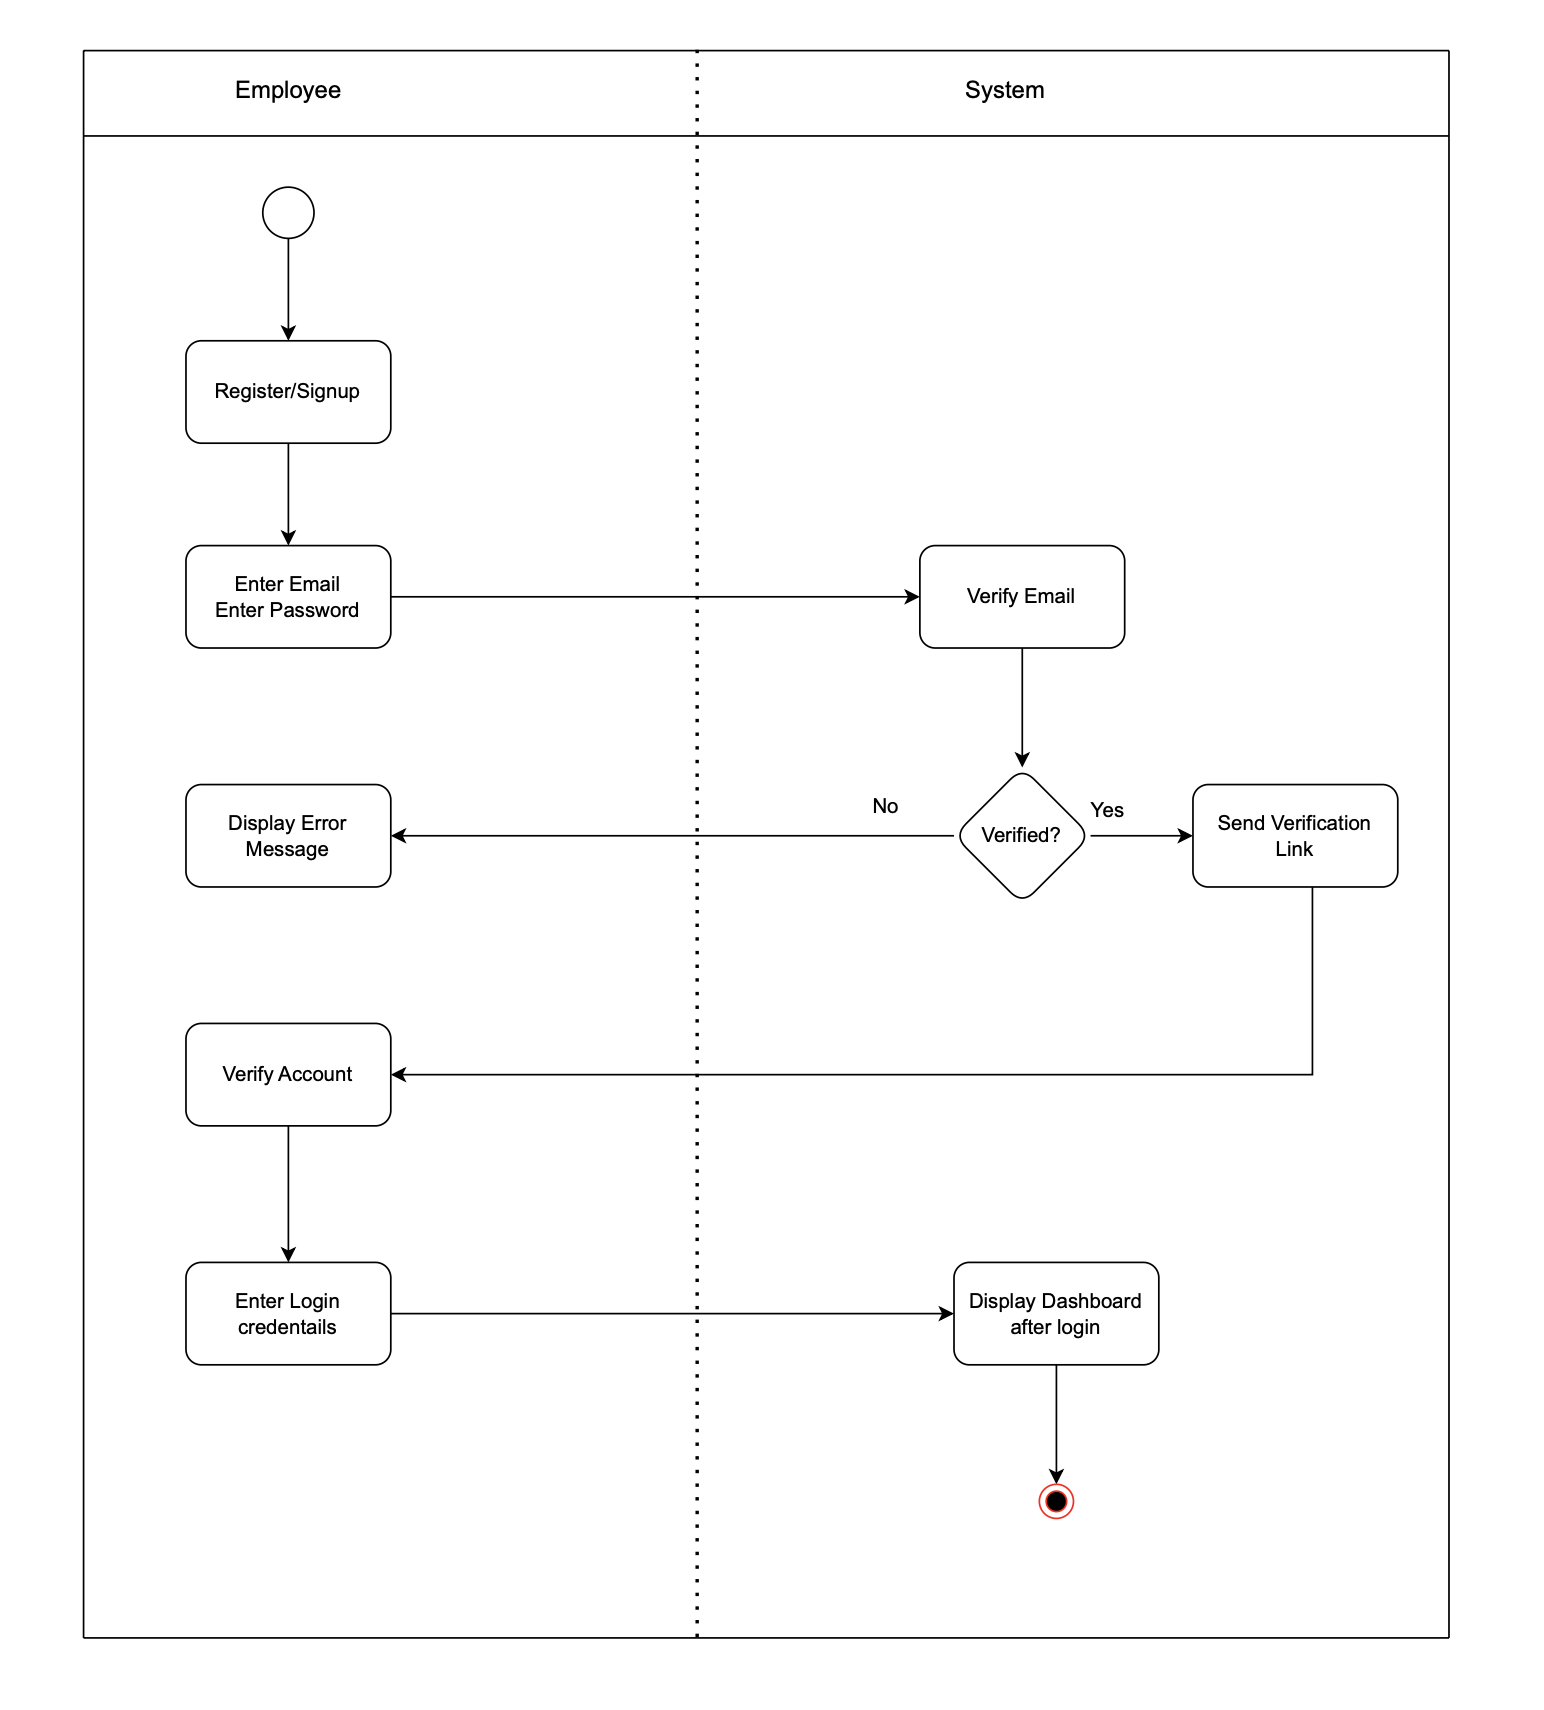
\includegraphics[width=\textwidth]{images/activityCreateAccount.png}
    \caption{Activity Diagram of Create Account use case}
    \label{fig:activityCreateAccount}
\end{figure}

\end{document}



\fancyhead[RO]{\textit{Part10}}
\chapter{Presentation}
Need to be added
\section{Section1}
Need to be added
\section{Section2}
Need to be added

\FloatBarrier
\newpage

\end{document}